\begin{frame}
\frametitle{About This Work...}

\emph{Learning-Based Cleansing for Indoor RFID Data}~\cite{baba2016learning}\\
A.I.~Baba, M.~Jaeger, H.~Lu, T.B.~Pedersen, W.-S.~Ku, X.~Xie.\\~\\

\begin{itemize}
  \item Published at \emph{SIGMOD' 2016}.
  \item Proposed a learning-based data cleansing approach that, requires no detailed prior knowledge about the spatio-temporal properties of the indoor space and the RFID reader deployment.
  \item Proposed the Indoor RFID Multi-variate Hidden Markov Model (IR-MHMM) to capture the uncertainties of indoor RFID data as well as the correlation of moving object locations and object readings.
\end{itemize}

\end{frame}

%------------------------------------------------

\begin{frame}
\frametitle{Motivation}

\begin{itemize}
  \item Recently there has been a remarkable proliferation of RFID in indoor tracking and monitoring systems
  \begin{fitemize}
    \item airport baggage monitoring. ~\cite{baba2013spatiotemporal,baba2013graph}
  \end{fitemize}
  \item The dirtiness of RFID data poses challenges to high-level RFID data querying and analysis.~\cite{chen2010leveraging}
  \begin{fitemize}
    \item \conceptbf{false negatives} (missing readings) occur when a reader fails to read a tag in its detection range.
    \item \conceptbf{false positives} (cross readings) occur when a tagged object is unexpectedly read by multiple readers simultaneously.
  \end{fitemize}
  \item This work focuses on cleansing \emph{false negatives} and \emph{false positives}.
\end{itemize}

\end{frame}

%------------------------------------------------

\begin{frame}
\frametitle{False Negatives \& False Positives}

\begin{columns}

  \column{0.4\textwidth}
  \begin{figure}[tb]
    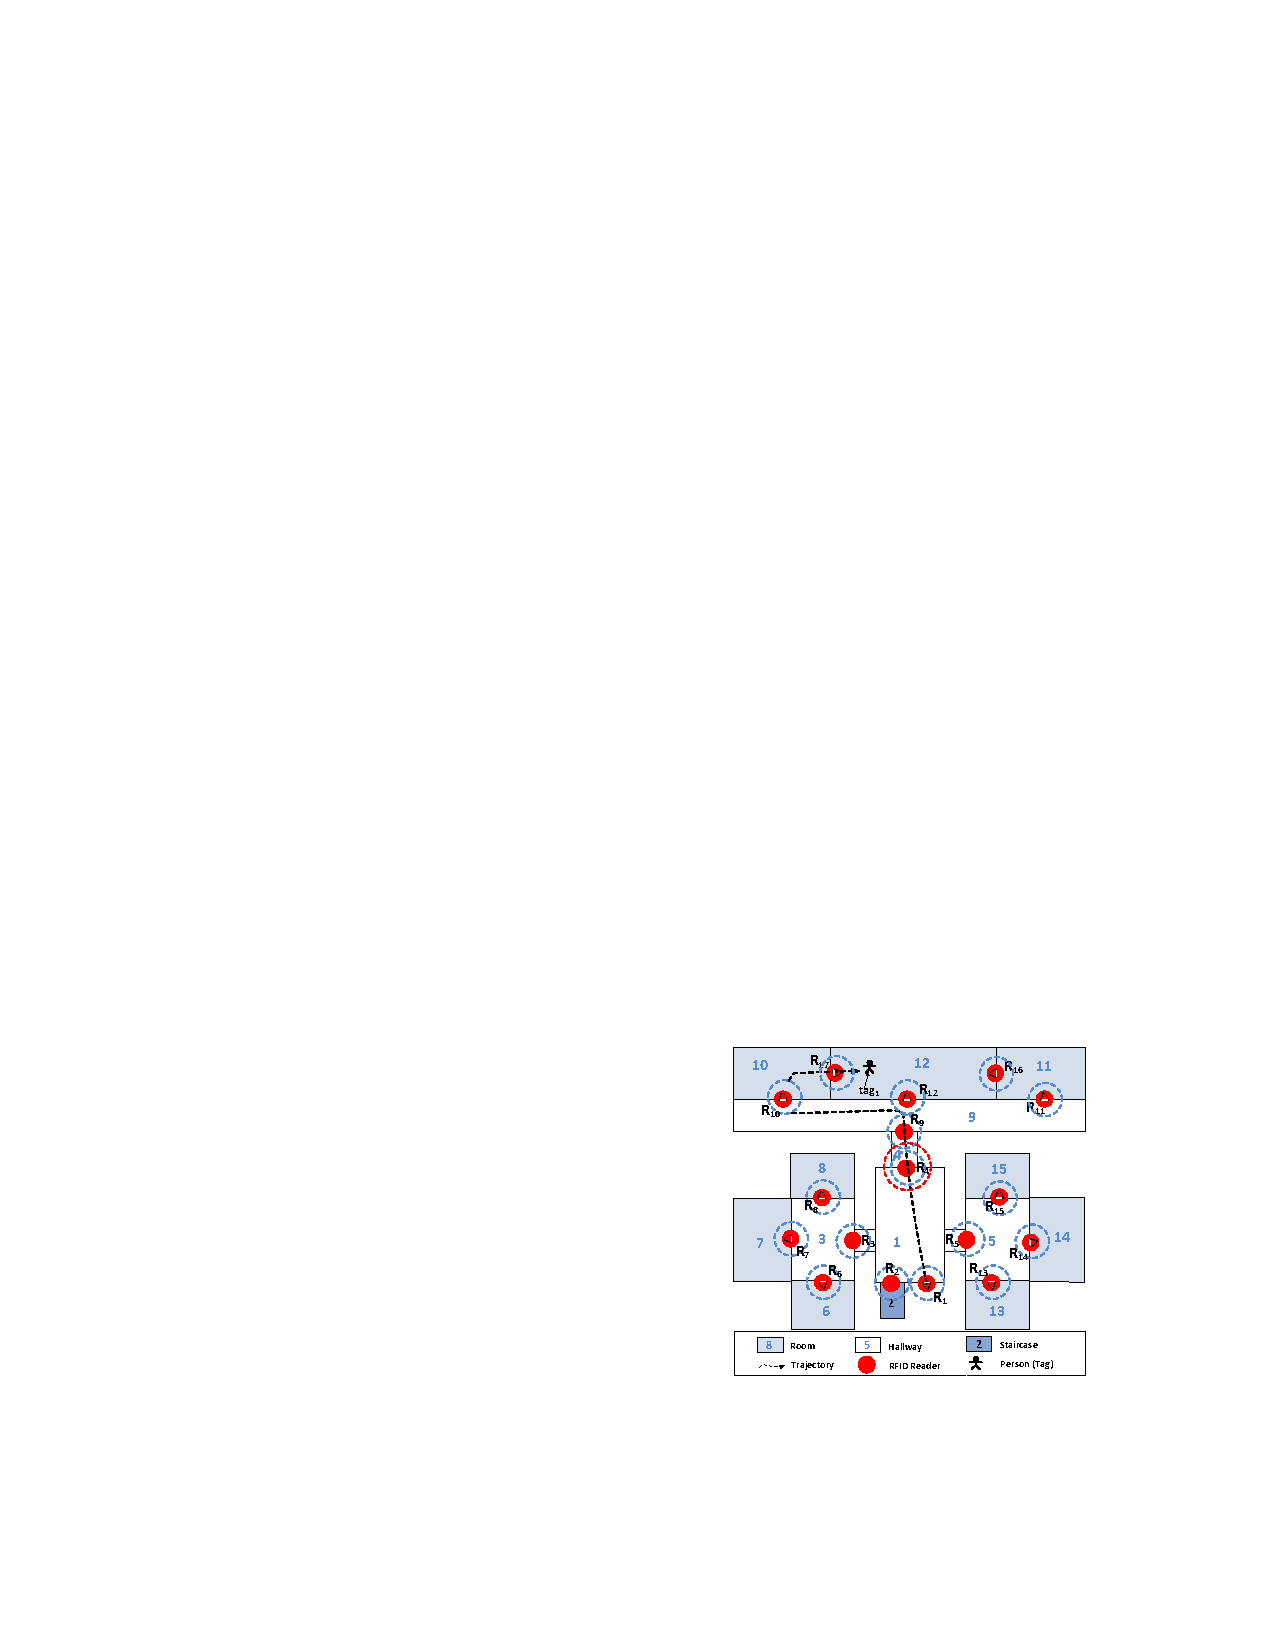
\includegraphics[width=\columnwidth]{figures/3-5/3-5-1.pdf}
  \end{figure}
  \ssize{\textit{an object with tag $tag_1$ moved into the building and was first detected by reader $R_1$ from time point $t_0$ to time point $t_3$, yielding four observations by reader $R_1$.}}

  \column{0.6\textwidth}
  \begin{figure}[tb]
    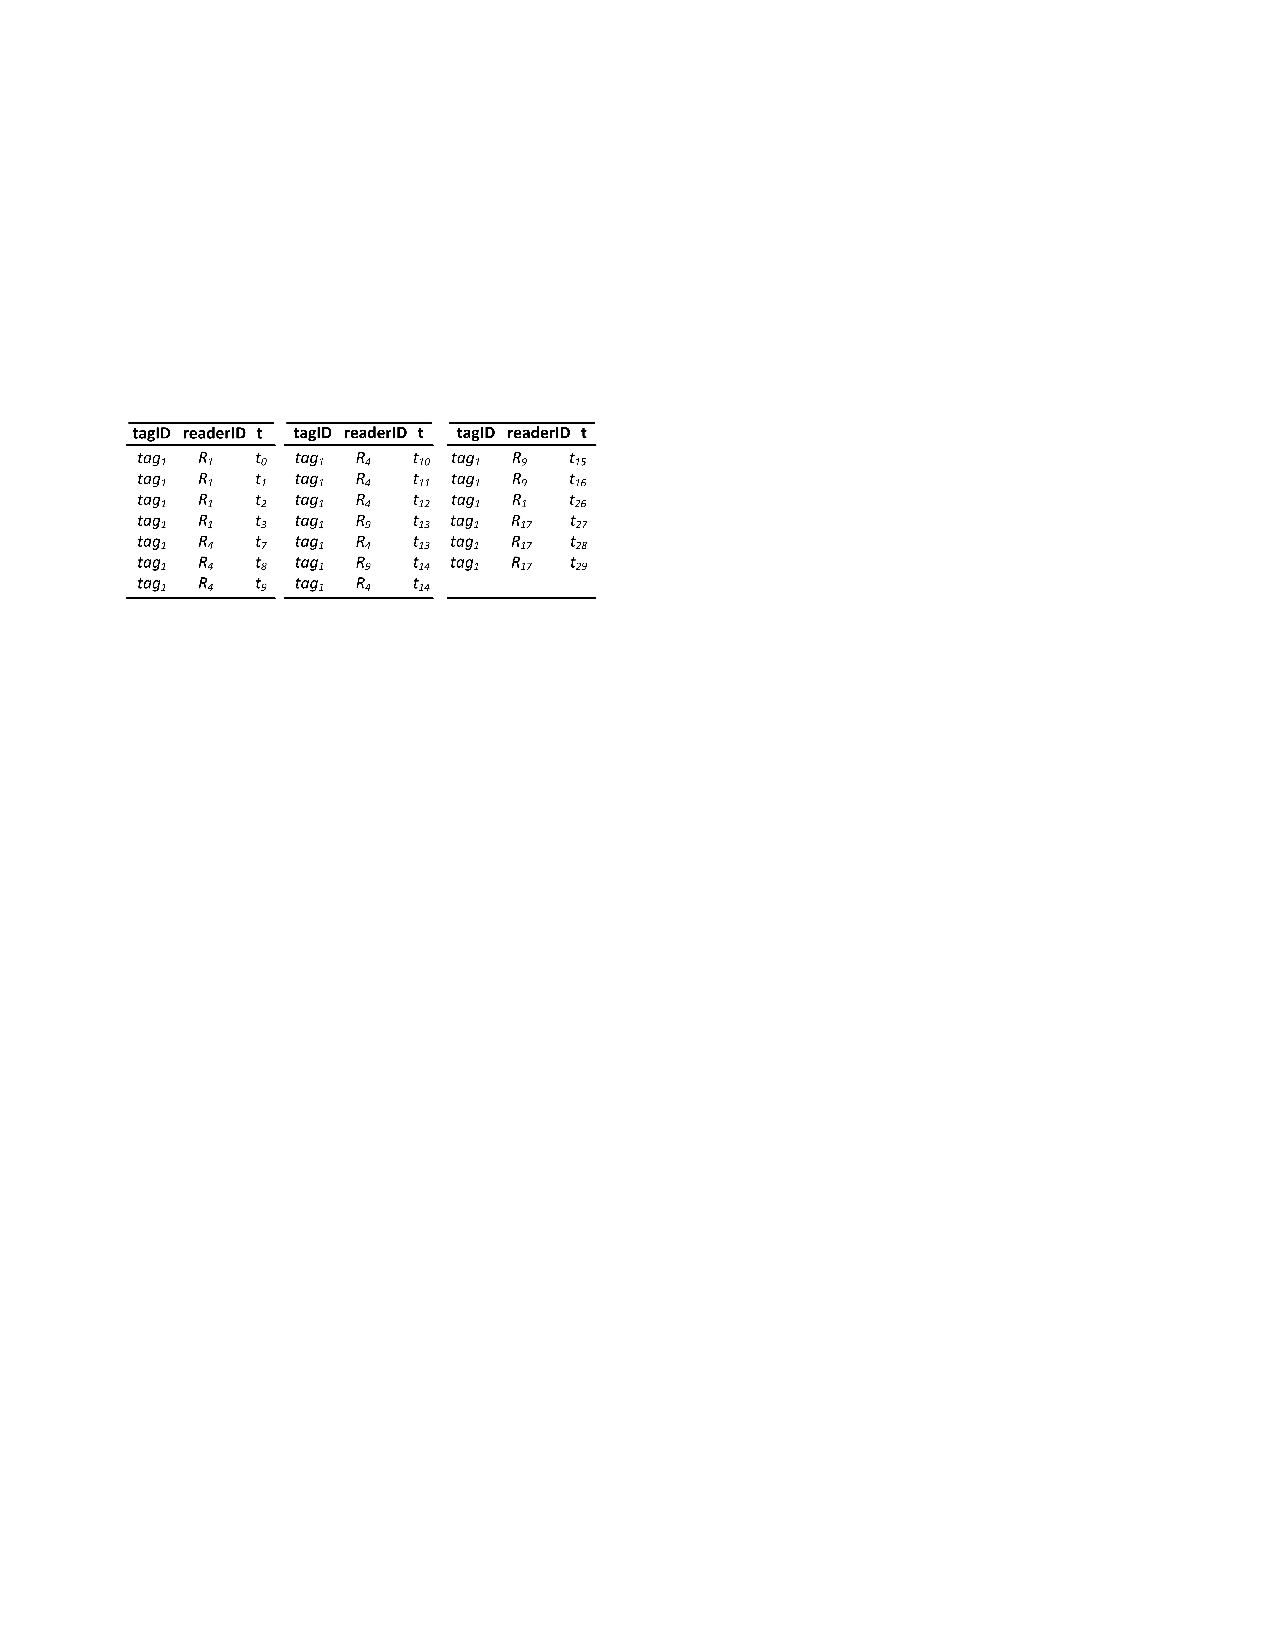
\includegraphics[width=\columnwidth]{figures/3-5/3-5-2.pdf}
  \end{figure}
  \ssize{
    1. at $t_{12}$ and $t_{13}$, $tag_1$ was detected by readers $R_4$ and $R_9$, it seems to be present in both locations, thus giving rise to a \emph{false positives}.\\~\\
    2. after $t_{16}$, $tag_1$ was detected by reader $R_{17}$ that kept detecting $tag_1$ until $t_{29}$. However $tag_1$ is not supposed to be detected by $R_{17}$ before it's detected by $R_{10}$. $tag_1$ passed through $R_{10}$ but failed to generate any information, giving rise to \emph{false negatives}.
  }

\end{columns}

\end{frame}

%------------------------------------------------

\begin{frame}
\frametitle{Motivation}

To support high-level RFID business logic processing, it is necessary to perform data cleansing to remove false negatives and false positives.\\~\\

Existing RFID data cleansing techniques require considerable specific prior knowledge for cleansing operations.

\begin{sitemize}
  \item to cleanse historical indoor RFID data, the graph model based cleansing approaches~\cite{baba2013spatiotemporal,baba2013graph,DBLP:conf/edbt/FazzingaFFP14} rely on graphs that capture the indoor topology, the deployment of readers, and multiple pertinet spatial-temporal properties.
  \item in the context of streaming RFID data, a probabilistic approach~\cite{tran2009probabilistic} demands to build four domain-specific probabilistic models before any data cleansing.
  \item also streaming RFID data, ~\cite{nie2009probabilistic} assumes that locations of neighboring objects are correlated to each other, lifting such assumptions and needs only minimal prior knowledge about indoor settings.
\end{sitemize}

\end{frame}

%------------------------------------------------

\begin{frame}
\frametitle{Preliminaries}

\ssize{\conceptbf{Hidden Markov Models} (HMMs) models two connected (discrete time) stochastic processes: an un-observed state transition process, and an observation process consisting of observable signals generated at each state. The underlying (hidden) state transition process is assumed to be Markovian and stationary.}

\begin{definition}[Hidden Markov Models]
  \ssize{
  An HMM is a tuple $\lambda = (\mathcal{S}, \mathcal{O}, A, B, \pi)$.
  \begin{enumerate}
    \item $\mathcal{S} = \{ s_1, ..., s_N \}$ is a set of (hidden) states.
    \item $\mathcal{O} = \{ o_1, ..., o_K \}$ is a set of possible observations.
    \item $A$ is an $N \times N$ transition probability matrix: $A = (a_{ij})_{i,j=1,...,N}$, where $a_{ij}$ represents the transition probability form hidden state $s_i$ to hidden $s_j$.
    \item $B$ is an $N \times K$ observation probability matrix: $B = (b_{ih})_{i=1,...,N;h=1,...K}$, where $b_{ih}$ is the probability of ovserving $o_h$ when the hidden process is in state $s_i$.
    \item $\pi$ is a $N$-dimensional initial state probability vector: $\pi = (\pi_i)_{i=1,...,N}$, where $\pi_i$ is the probability that the hidden state process starts in state $s_i$.
  \end{enumerate}
  }
\end{definition}

\end{frame}

%------------------------------------------------

\begin{frame}
\frametitle{Preliminaries}

An HMM defines a discrete time stochastic process over the combined state and observation space $\mathcal{S} \times \mathcal{O}$. \\~\\

The state of the process at time $t$ is described by \emph{random variables} $S^{(t)}$ with values in $\mathcal{S}$, and $\mathcal{O}^{(t)}$ is defined by

\pause
\begin{equation}
  P(S^{(0)} = s_i) = \pi_i
\end{equation}

\pause
\begin{equation}
  P(S^{(t+1)} = s_j | S^{(t)} = s_i) = a_{ij}
\end{equation}

\pause
\begin{equation}
  P(o^{(t)} = o_h | S^{(t)} = s_i) = b_{ih}
\end{equation}

\end{frame}

%------------------------------------------------

\begin{frame}
\frametitle{Preliminaries}

For modeling processes where at each point in time observations of multiple variables are made, the basic HMM model have been generalized to \conceptbf{Multi-variate Hidden Markov Models}(MH-MMs).~\cite{kirshner2005modeling}.\\~\\

The simple observation space $\mathcal{O}$ is replaced by a multivariate observation space $\mathcal{O}_1 \times \hdots \times \mathcal{O}_M$, and at each time $t$ one observes variables $O^{(t)}_1,...,O^{(t)}_M$.\\~\\

One can furthermore introduce the assumption that the different observations are \emph{independent} given the hidden state, i.e.,

\pause

\begin{equation}
  P(O^{(t)}_1,...,O^{(t)}_M | S^{(t)}) = \prod_{i=1}^M P(O^{(t)}_i | S^{(t)})
\end{equation}

\end{frame}

%------------------------------------------------

\begin{frame}
\frametitle{Data Transformation}

\textbf{Discretize the contunuous timestamp data} \quad for the duration $(t_e - t_s)$, a time granularity $\alpha$ is chosen to spans the discrete time points $0,...,(T-1)$, where $T = \frac{t_e - t_s}{\alpha}$.\\~\\

A continuous time record $\langle readerID, t \rangle$ is replaced by $\langle readerID, i \rangle$ where $i$ is such that $t \in [t_s + i * \alpha, t_s +(i+1) * \alpha]$.


\end{frame}

%------------------------------------------------

\begin{frame}
\frametitle{Data Transformation}

\textbf{Choice of $\alpha$} --
\begin{itemize}
  \item it should be chosen small enough so that discretization does not introduce any spurious appearances of cross readings, this can be ensured when $\alpha < \Delta_{min} / 2$, where $\Delta_{min}$ is the minimum absolute difference between continuous time-stamps of records with different $readID$s.
  \item the time granularity must be small enough so that clean data of this granularity is sufficient for subsequent tracking and analysis purposes.
  \item under the above constraints, it should be as large as possible, to minimize the computational complexity.
\end{itemize}

\end{frame}

%------------------------------------------------

\begin{frame}
\frametitle{Data Transformation}

\begin{columns}

  \column{0.55\textwidth}
  \begin{figure}[tb]
    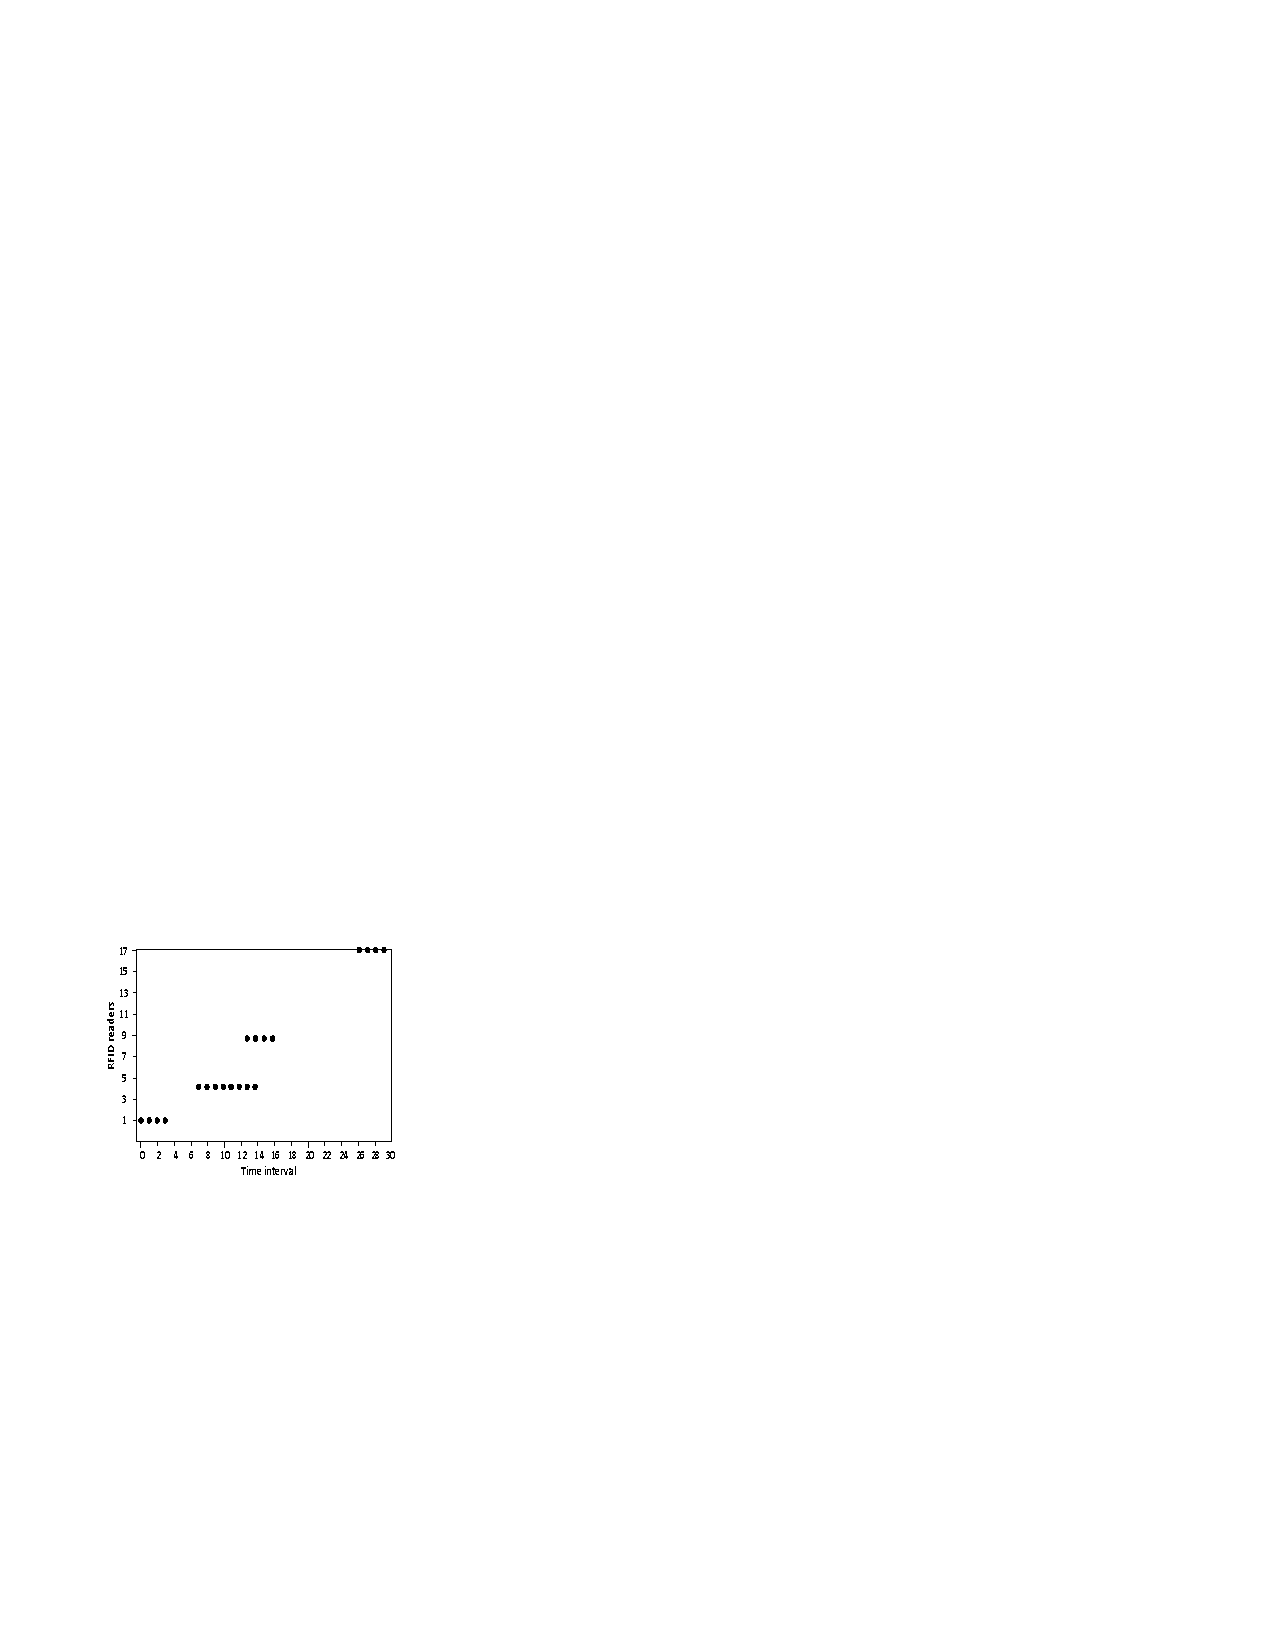
\includegraphics[width=0.7\columnwidth]{figures/3-5/3-5-3.pdf}
  \end{figure}
  \fsize{this figure shows an alternative representation of discretized data, time points and possible reader IDs are on the $x$ and $y$-axis respectively.}

  \column{0.45\textwidth}
  \begin{figure}[tb]
    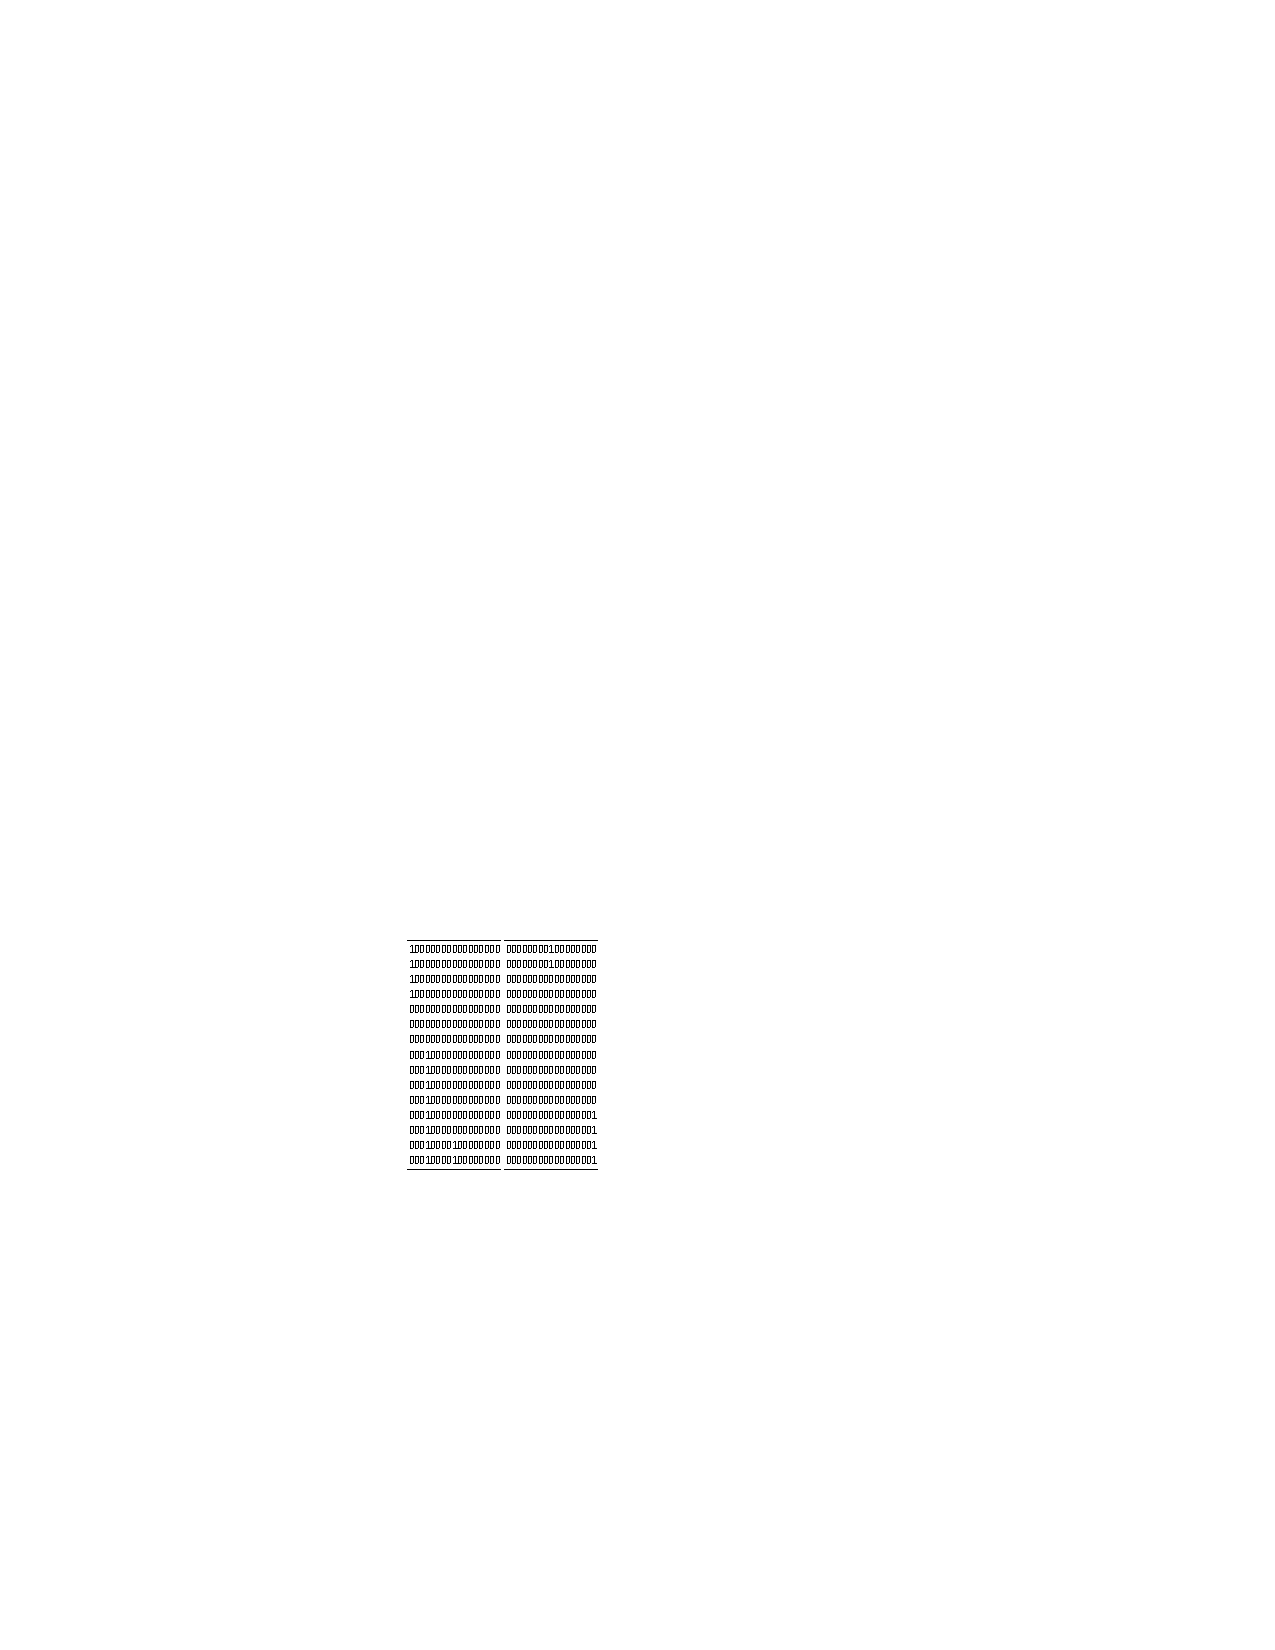
\includegraphics[width=0.7\columnwidth]{figures/3-5/3-5-4.pdf}
  \end{figure}
  \fsize{this figure equivalently encodes left figure's data as a sequence of $T$ binary vectors of length $M$, where $M$ is the number of readers.}

\end{columns}

\end{frame}

%------------------------------------------------

\begin{frame}
\frametitle{Data Transformation}

At the end of the transformation process, the data consists of a sequence $\mathbf{V}_r^{(0)}$,...,$\mathbf{V}_r^{(T-1)}$, where each $\mathbf{V}_r^{(t)} \in \{ 0, 1 \}^M$. (\textit{subsript $r$ stands for ``raw''}) \\~\\

The $k$th component of $\mathbf{V}_r^{(t)}$ is denoted as $\mathbf{V}_{r,k}^{(t)}$. \\~\\

Consider the $\mathbf{V}_r^{(t)}$ as the observations in a MHMM process, and use standard HMM learning and inference techniques to transform the $\mathbf{V}_r^{(t)}$ into cleaned versions $\mathbf{V}_c^{(t)}$. \\~\\

The cleaned data still takes values in $\{ 0, 1 \}^M$, but with the condition that each $\mathbf{V}_c^{(t)}$ contains at most one non-zero entry (i.e., no cross readings).

\end{frame}

%------------------------------------------------

\begin{frame}
\frametitle{Probabilistic Inference for RFID Streams}

Given a sequence of raw readings $\mathbf{o}_r = o^{(0)}_r,...,o^{(T-1)}_r$, where each $o^{(t)}_r$ is an observation of a random variable $O^{(t)}_r$ that takes values in a raw observation space $\mathcal{O}_r$. \\~\\

From $\mathbf{o}_r$ we want to infer a clean data sequence $\mathbf{o}_c = o^{(0)}_c,...,o^{(T-1)}_c$ of observations of random variables $O^{(t)}_c$ that takes values in a clean observation space $\mathcal{O}_c$. \\~\\

Based on a probabilistic model for $\mathbf{O}_r$ and $\mathbf{O}_c$ one can infer the clean from the raw data $\mathbf{o}_r$ by selecting the $\mathbf{o}_c$ that maximizes the conditional probability $P(\mathbf{O}_c = \mathbf{o}_c | \mathbf{O}_r = \mathbf{o}_r)$. \\~\\

\end{frame}

%------------------------------------------------

\begin{frame}
\frametitle{Probabilistic Inference for RFID Streams}

\textit{A straightforward approach to defining the joint distribution of $\mathbf{O}_r$, $\mathbf{O}_c$} is in the form of an HMM with $O^{(t)}_r$ as the observable variables, and $O^{(t)}_c$ as the hidden state variables $S^{(t)}$.

\begin{itemize}

  \item the first difficulty lies in the fact that the hidden state space \emph{must correspond to} the clean observation space that is required for the RFID data stream processing.

  \item the second difficulty arising from equating $\mathcal{S} = \mathcal{O}_c$ lies in constructing or learning an \emph{adequate model}.

\end{itemize}

\end{frame}

%------------------------------------------------

\begin{frame}
\frametitle{The First Difficulty}

On the basis of the particular hidden state space, and under the limitation of the Markov assumption for the \emph{state transition model}, it may not be possible to obtain an accurate model for the joint distribution $P(\mathbf{O}_c, \mathbf{O}_r)$.\\~\\

\begin{example}
  \ssize{
  Consider the concrete raw and clean data model $\mathbf{V}^{(t)}_r, \mathbf{V}^{(t)}_c \in \{ 0,1 \}^M$, the clean state $0^M$ (no reading) would be a hidden HMM state;\\

  Under the Markov assumption, the model could \emph{not} represent that given that currently there is no reading, the probability distribution over the next reading depends on what the most recent available reading has been.\\
  }
\end{example}

\end{frame}

%------------------------------------------------

\begin{frame}
\frametitle{The Second Difficulty}

Since now inferred hidden state sequences are the target of inference, one has to ensure that inferred hidden state values actually correspond to the relevant properties of the underlying tracking process that we want to capture with the clean data $\mathbf{O}_c$.\\~\\

\conceptbf{Semantic States} are the hidden HMM states that are endowed in the manner with an intended meaning.\\~\\

Constuction of HMMs whose hidden states adhere to intended semantics usually requires either manual design, or learning from labeled training data in which besides the observation variables $\mathbf{O}$ also the hidden states $\mathbf{S}$ are given.

\end{frame}

%------------------------------------------------

\begin{frame}
\frametitle{Unsupervised Learning based Construction of HMMs}

\conceptbf{The goal} of this work is  to construct HMMs for $P(\mathbf{O}_c | \mathbf{O}_r)$ in a completely unsupervised manner, i.e., by learning from training data that consists of the raw observations $\mathbf{O}_r$ only.\\~\\

The hidden state space $\mathcal{S}$ consists of \conceptbf{latent states}: states that have no pre-defined interpretation, and that are only introduced to support an adequate Markov model for the variables of $\mathbf{O}_c$, $\mathbf{O}_r$.\\~\\

To define a joint distribution $P(\mathbf{S}, \mathbf{O}_r, \mathbf{O}_c)$, making a natural conditional independence assumption between $\mathbf{O}_r$ and $\mathbf{O}_c$ given $\mathbf{S}$: \pause

\begin{equation}
  P(\mathbf{S}, \mathbf{O}_r, \mathbf{O}_c) = P(\mathbf{S}) P(\mathbf{O}_r | \mathbf{S}) P(\mathbf{O}_c | \mathbf{S})\label{equation:joint_prob_model}
\end{equation}

\end{frame}

%------------------------------------------------

\begin{frame}
\frametitle{Unsupervised Learning based Construction of HMMs}

Given the model $P(\mathbf{S}, \mathbf{O}_r, \mathbf{O}_c)$, the data cleaning inference task is to compute for a given observed raw data sequence $\mathbf{o}_r$: \pause

\begin{equation}
  \begin{split}
  & \arg\max\limits_{\mathbf{o}_c} P(\mathbf{O}_c = \mathbf{o}_c | \mathbf{O}_r = \mathbf{o}_r) = \\
  & \sum_{\mathbf{s}} P(\mathbf{S} = \mathbf{s} | \mathbf{O}_r = \mathbf{o}_r) P(\mathbf{O}_c = \mathbf{o}_c | \mathbf{S} = \mathbf{s})
  \end{split}\label{equation:inference_task}
\end{equation}

\pause

Here the sum is over all hidden state sequences $\mathbf{s}$ of the same length as $\mathbf{o}_r$.

\end{frame}

%------------------------------------------------

\begin{frame}
\frametitle{The First Challenge}

\begin{block}{Challenge 1}
  it is to learn the model Equation.\ref{equation:joint_prob_model}, which includes the conditional distribution $P(\mathbf{O}_r | \mathbf{S})$ containing only variables for which there is no observations at all.
\end{block}

\vspace{10pt}

Tackle the above challenge by making some strong assumptions on the relationship between $\mathbf{O}_c$ and $\mathbf{O}_r$. \\~\\

The first assumption is that the clean data space is a subset of the raw data space: $\mathcal{O}_c \subseteq \mathcal{O}_r$. The assumption is true in the specific data model, where $\mathcal{O}_r = \{ 0,1 \}^M$, and $\mathcal{O}_c \subseteq \mathcal{O}_r$ consists of the vectors with at most one non-zero component.


\end{frame}

%------------------------------------------------

\begin{frame}
\frametitle{The First Challenge}

A crucial assumption is then made. Intuitively, assume that $\mathbf{O}_r$ and $\mathbf{O}_c$ are generated by the same random process given $\mathbf{S}$, only that $\mathbf{O}_c$ is conditioned on the subset $\mathcal{O}_c$: \pause

\begin{equation}
  \begin{split}
  & P(\mathbf{O}_c = \mathbf{o}_c | \mathbf{S} = \mathbf{s}) = \\
  & P(\mathbf{O}_r = \mathbf{o}_c | \mathbf{S} = \mathbf{s}) / P(\mathbf{O}_r \in \mathcal{O}_c^T | \mathbf{S} = \mathbf{s})
  \end{split}
\end{equation}

\end{frame}

%------------------------------------------------

\begin{frame}
\frametitle{The Second Challenge}

\begin{block}{Challenge 2}
  the maximization of Equation.\ref{equation:inference_task} should be solved efficiently.
\end{block}

\vspace{10pt}

\fsize{

Following the last slide, the inference problem becomes to compute: \pause

\begin{equation}
  \arg\max\limits_{\mathbf{o}_c \in \mathcal{O}_c^T} \sum_{\mathbf{s}} \frac{P(\mathbf{S} = \mathbf{s} | \mathbf{O}_r = \mathbf{o}_r) P(\mathbf{O}_r = \mathbf{o}_c | \mathbf{S} = \mathbf{s})}{P(\mathbf{O}_r \in \mathcal{O}_c^T | \mathbf{S} = \mathbf{s})}
\end{equation}

\pause

\vspace{10pt}

The summation over all hidden states sequences $\mathbf{s}$ will be computationally infeasible, therefore, it should approximate the posterior distribution $P(\mathbf{S} = \mathbf{s} | \mathbf{O}_r = \mathbf{o}_r)$ by only considering the most probable state $\mathbf{\hat{s}}= \arg \max_{\mathbf{s}}P(\mathbf{S} = \mathbf{s} | \mathbf{O}_r = \mathbf{o}_r)$ and then to compute: \pause

\begin{equation}
  \arg\max\limits_{\mathbf{o}_c \in \mathcal{O}_c^T} P(\mathbf{O}_r = \mathbf{o}_c | \mathbf{S} = \mathbf{\hat{s}})
\end{equation}

}

\end{frame}

%------------------------------------------------

\begin{frame}
\frametitle{Indoor RFID Multi-variate HMM}

\begin{definition}[Indoor RFID Multi-variate HMM (IR-MHMM)]
  \begin{equation*}
    \lambda = (\mathcal{S}, \{ 0,1 \}^M, A, B, \pi)
  \end{equation*}
  \fsize{
    $\mathcal{S}, A, \pi$ are as in the generic (M)HMM definition, and the observation space is $\mathcal{O} = \{ 0,1 \}^M$.\\
    Assuming that different readers are independent given the hidden state, the observation model is given by the probabilities $b_{ik} := P(V^{(t)}_{r,k} = 1 | S^{(t)} = s_i)$ (i.e., the probability of getting in the $i$th hidden state a reading from the $k$th reader).\\
    The observation model is now represented by a matrix $B$ of dimensions $N \times M$ with entries $b_{ik}$.
  }
\end{definition}

\begin{figure}[tb]
  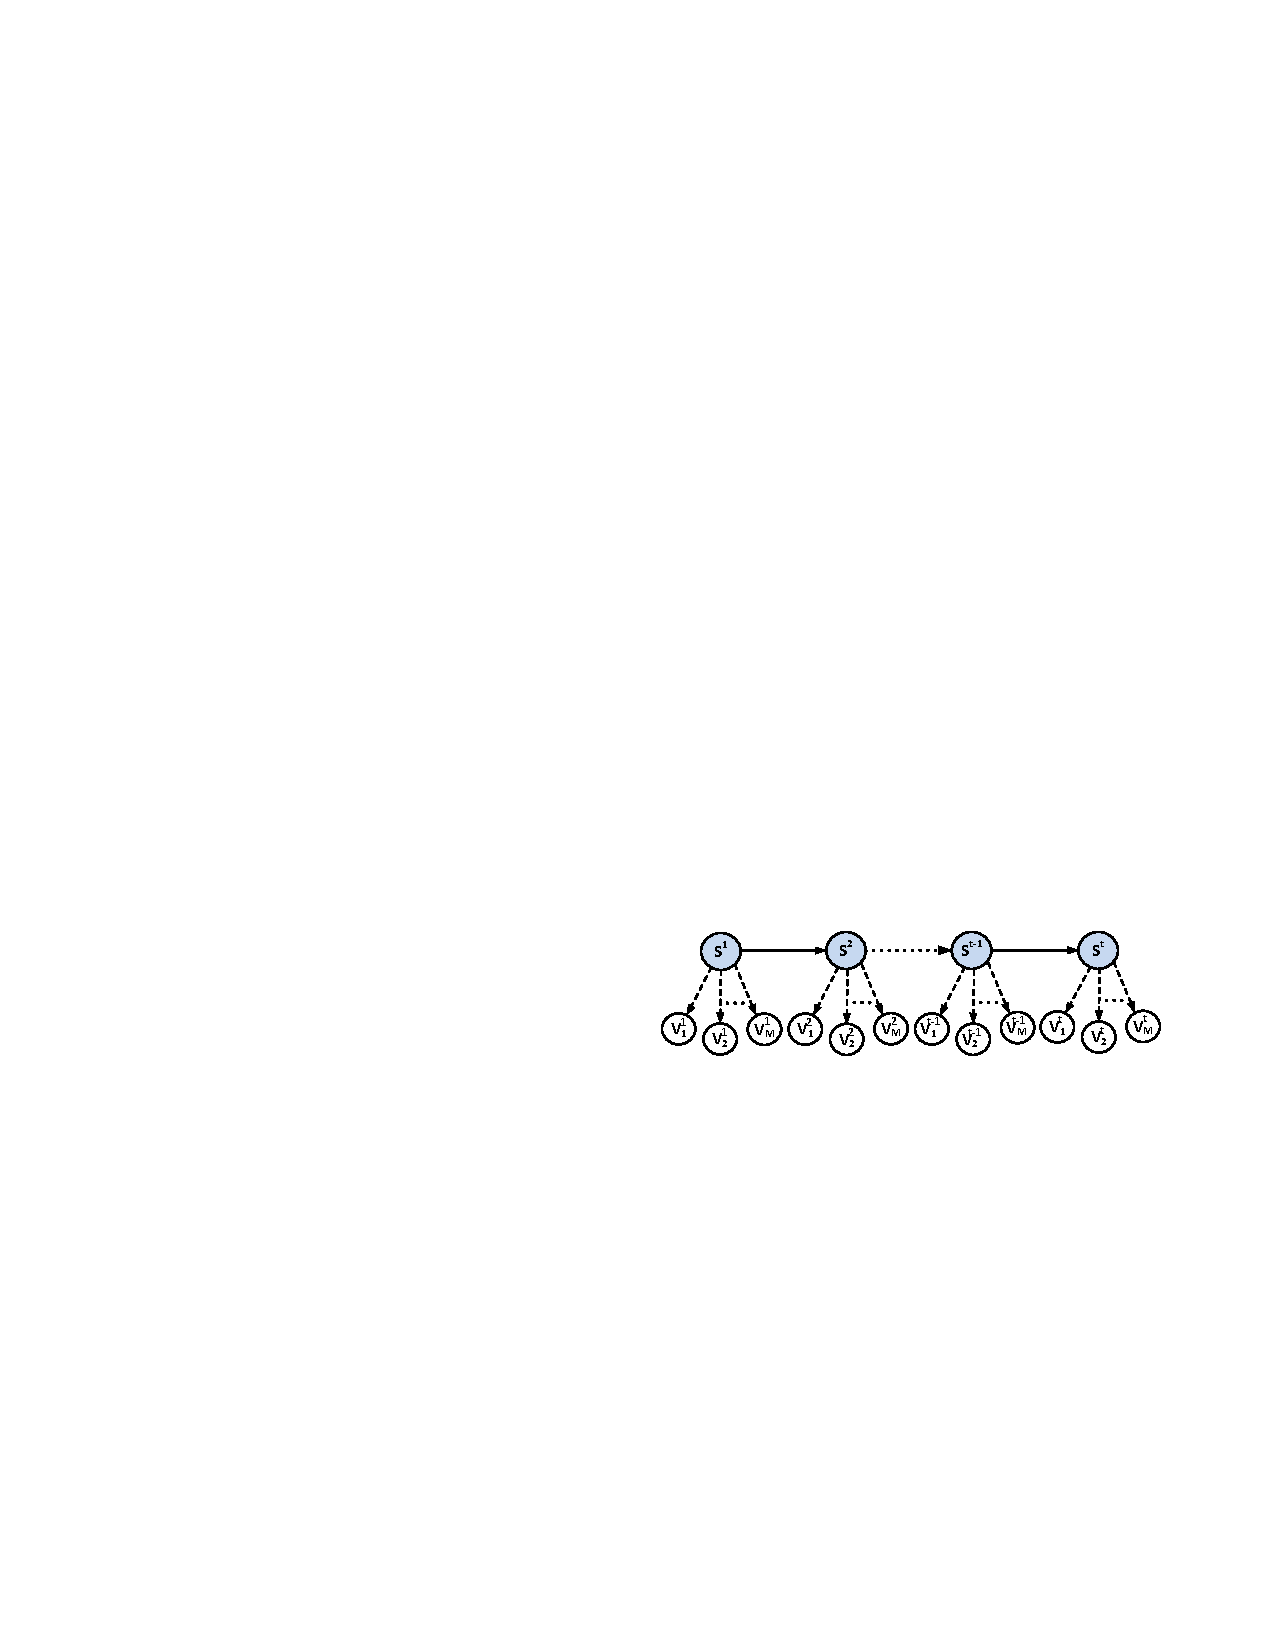
\includegraphics[width=0.7\columnwidth]{figures/3-5/3-5-5.pdf}
\end{figure}

\end{frame}

%------------------------------------------------

\begin{frame}
\frametitle{Construction: Overview}

The construction (modeling paramters $N, A, B, \pi$) is a combination of design and learning.
\begin{fitemize}
  \item to minimize the amout of domain specific information required in the design component (such as spatial distance, travel time etc.)
  \item to base the learning component entirely on learning from the raw data $\mathbf{V}_r$ without any further annotations.
\end{fitemize}

\begin{block}{}
  \ssize{
  \begin{enumerate}
    \item the cardinality $N$ of the state space is chosen in the design step.
    \item the states $s_i \in \mathcal{S}$ are purely latent, without any associated semantics a-priori. Only after learning may it be possible to assign a semantic interpretation to some states.
    \item however, the learning is from raw data that does not contain information about the true nature of hidden states, there is no guarantee that after learning the states closely adhere to their intended semantics.
  \end{enumerate}
  }
\end{block}

\end{frame}

%------------------------------------------------

\begin{frame}
\frametitle{Construction: State Space Design}

\begin{itemize}
  \item Four different state space designs for IR-MHMMs are proposed.
  \item All require as input at most some qualitative spatial information as expressed by a \emph{reader deployment graph}.
  \item Designs define a set of states with associated intended semantics such as:
    \begin{fitemize}
        \item states representing (approximate) spatial locations
        \item states representing some history of past transitions
    \end{fitemize}
  \item The intended semantics of hidden states lead to constraints of the form $a_{ij} = 0$ (for some combinations $i,j$ of states direct ransitions will not be possible).
\end{itemize}

\end{frame}

%------------------------------------------------

\begin{frame}
\frametitle{Minimum State Model (MSM)}

\begin{columns}

  \column{0.5\textwidth}
  \vspace{-10pt}
  \begin{figure}[tb]
    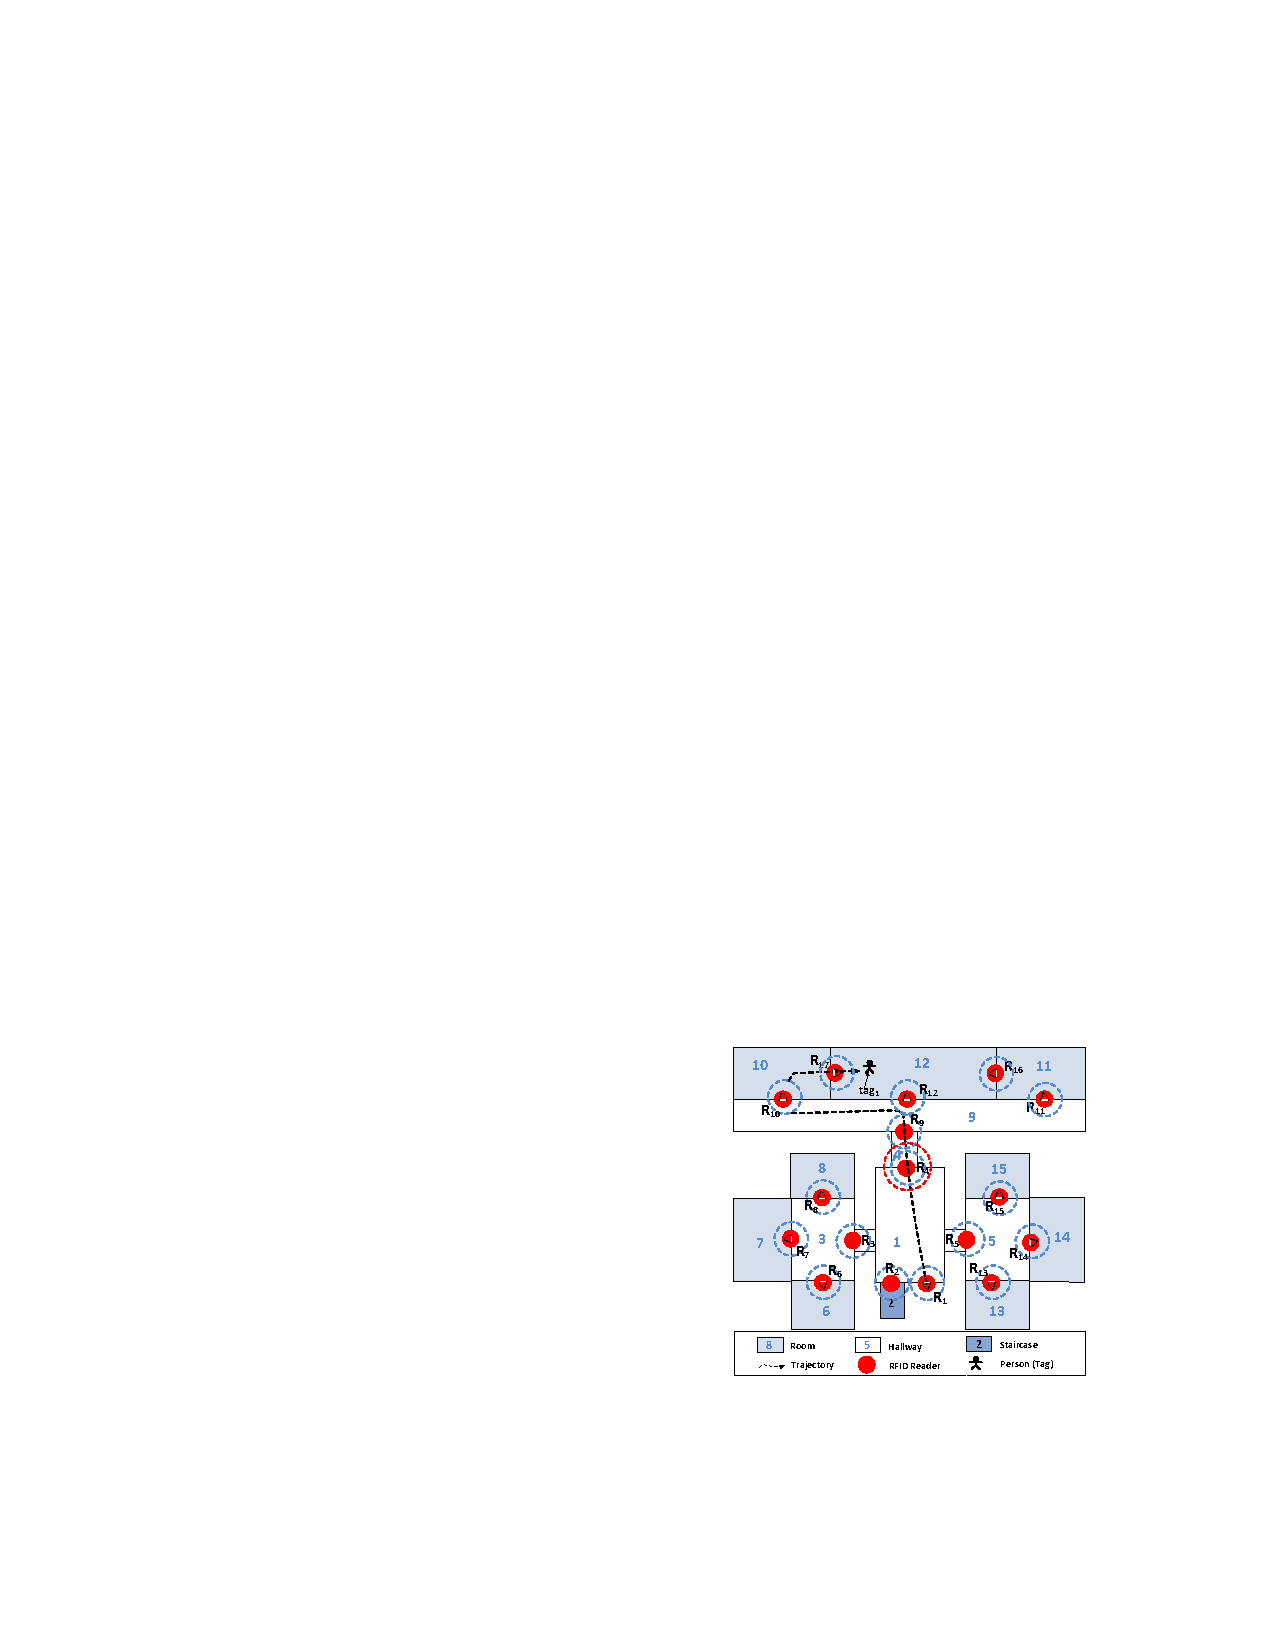
\includegraphics[width=0.75\columnwidth]{figures/3-5/3-5-1.pdf}
  \end{figure}
  \vspace{-20pt}
  \begin{figure}[tb]
    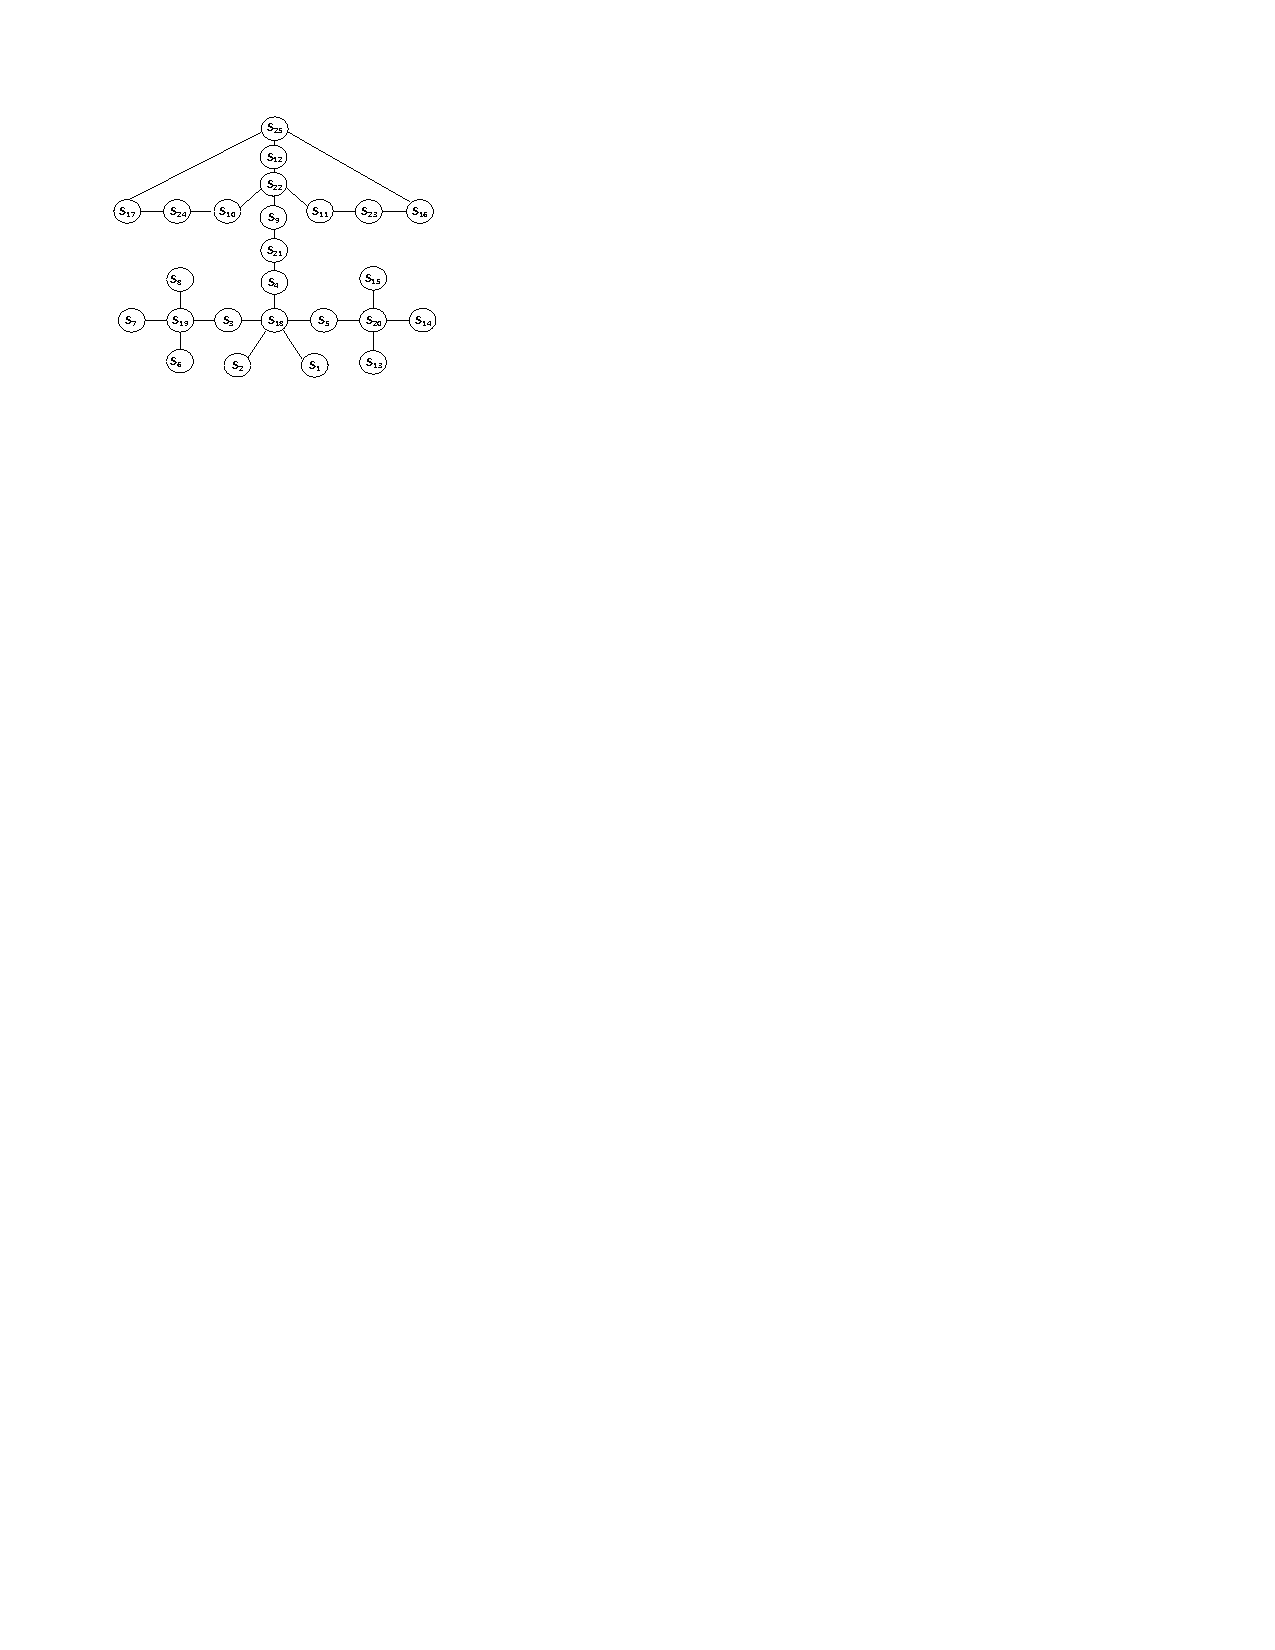
\includegraphics[width=0.75\columnwidth]{figures/3-5/3-5-6.pdf}
  \end{figure}

  \column{0.6\textwidth}
  \ssize{
  \textrm{This design contains a state for each deployed reader $R_i$, and a state for each hallway or any indoor partition that is connected with more than one reader.}\\~\\
  \begin{example}
    For example, reader $R_4$ is represented as state $s_4$. Furthermore, hallway 3 is connected with four readers $R_3, R_6, R_7, R_8$, thus it's represented by a state $s_{19}$. The total number of states in example is $N = 25$. The transition model is constrainted by setting $a_{ij} = 0$ if $s_i$ and $s_j$ correspond to locations that are not directly connected.
  \end{example}
  }
\end{columns}

\end{frame}

%------------------------------------------------

\begin{frame}
\frametitle{Last State Model (LSM)}

\begin{columns}

  \column{0.5\textwidth}
  \vspace{-10pt}
  \begin{figure}[tb]
    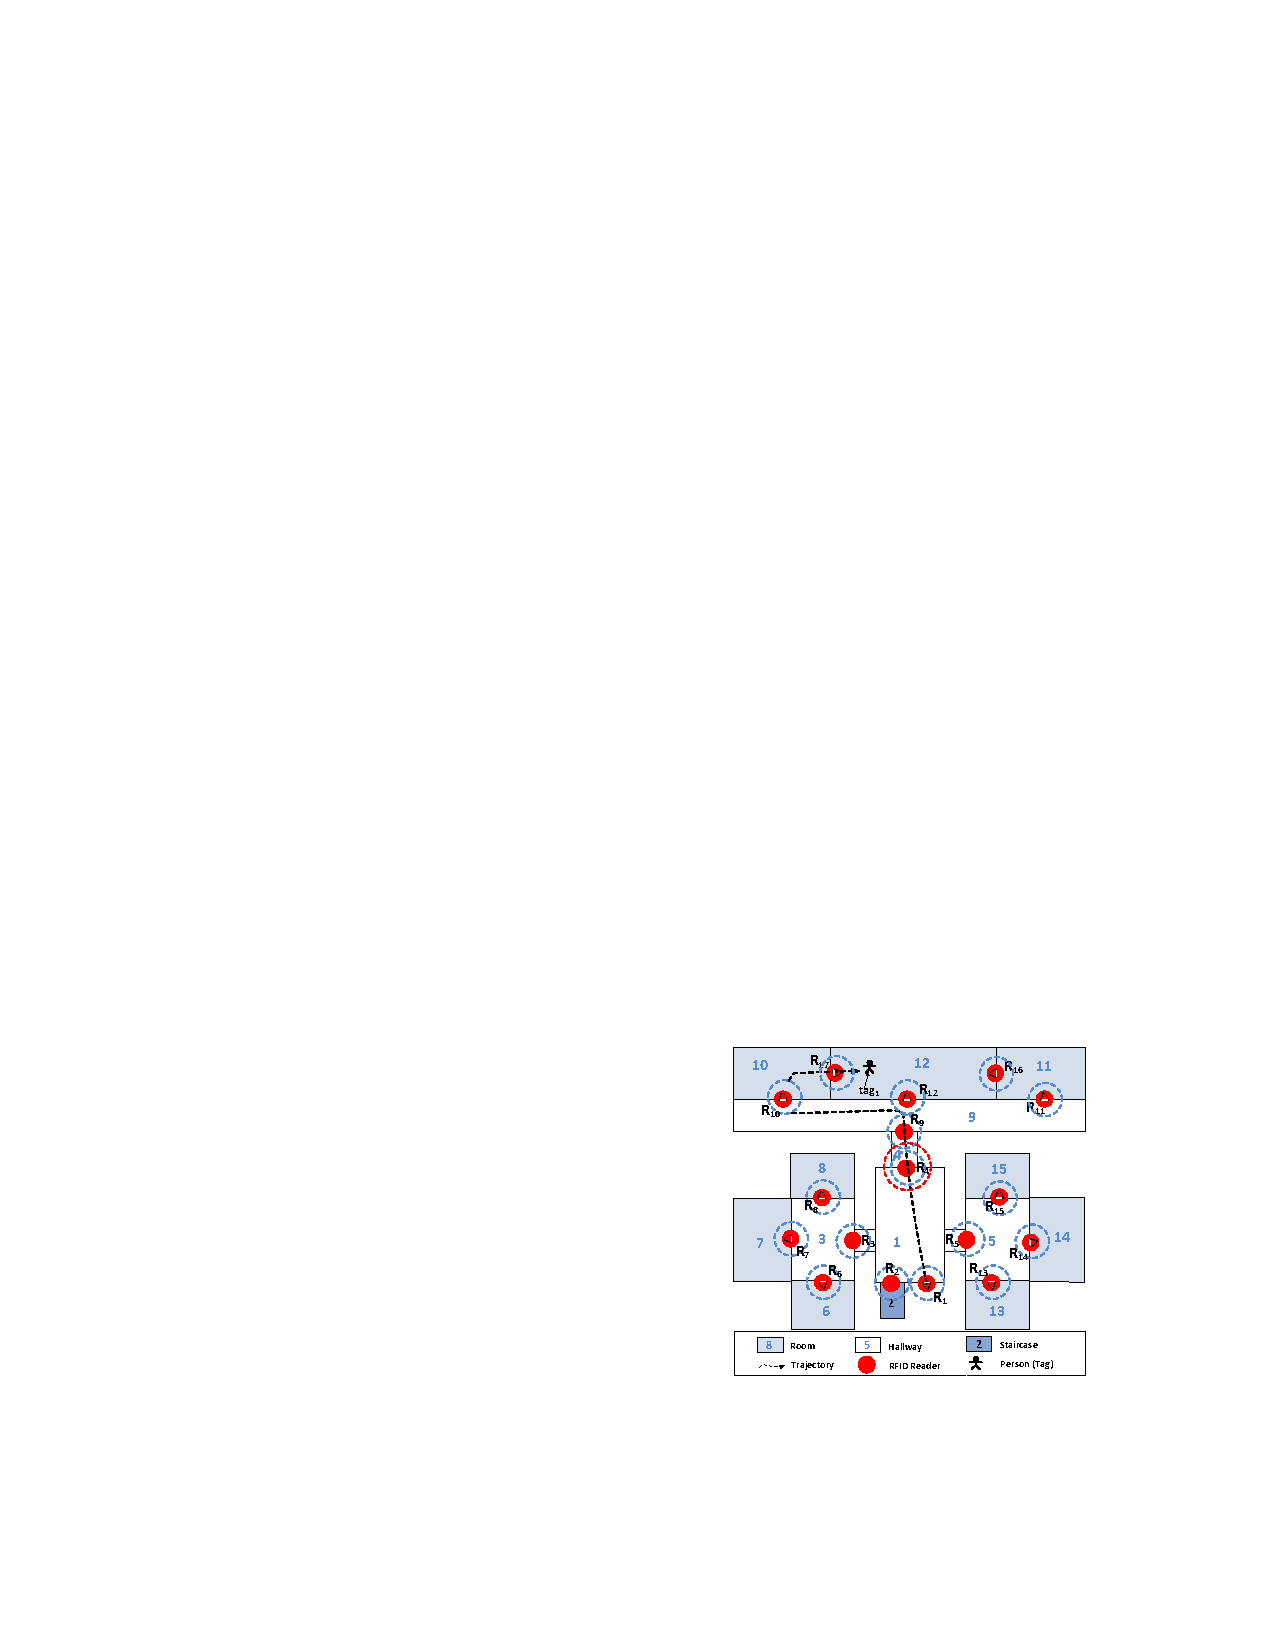
\includegraphics[width=0.75\columnwidth]{figures/3-5/3-5-1.pdf}
  \end{figure}
  \vspace{-20pt}
  \begin{figure}[tb]
    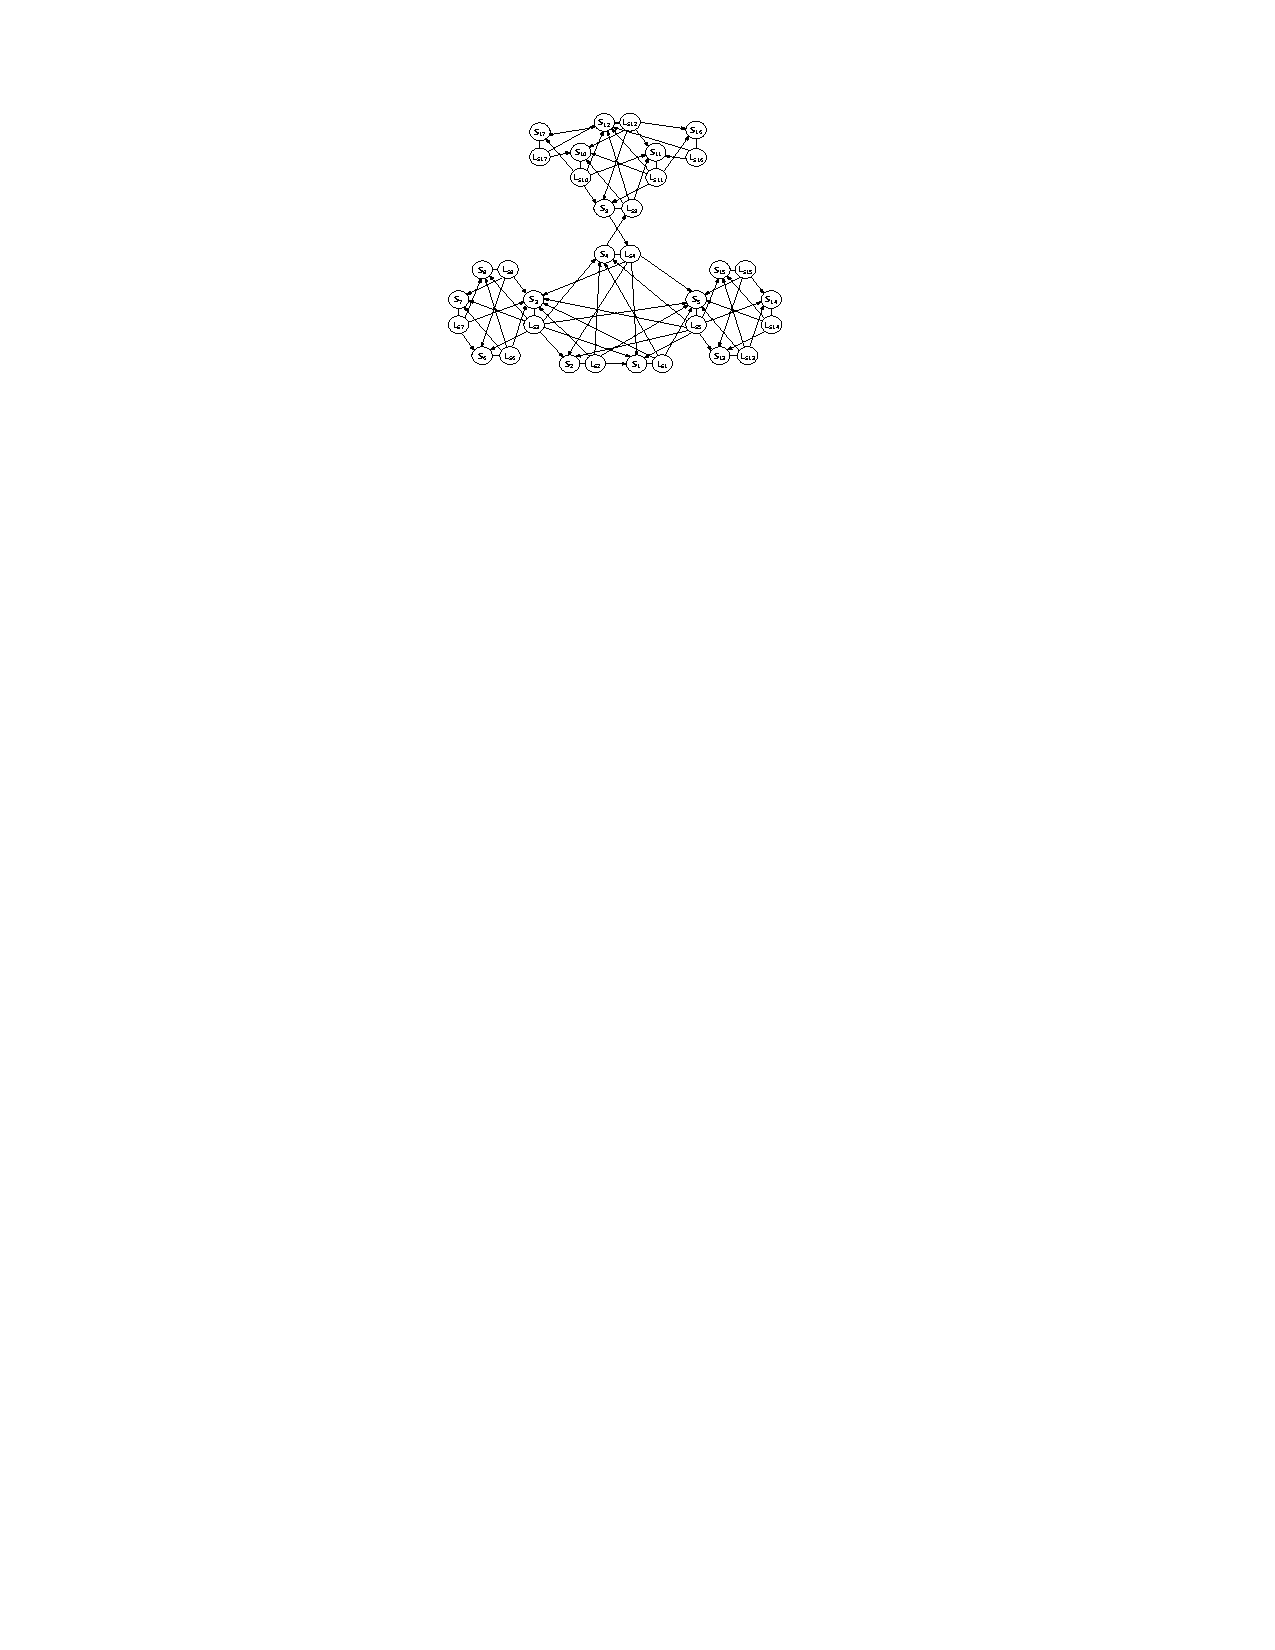
\includegraphics[width=0.75\columnwidth]{figures/3-5/3-5-7.pdf}
  \end{figure}

  \column{0.6\textwidth}
  \ssize{
  \textrm{This design contains two state $s_i$ and $l_{si}$ for each deployed reader $R_i$. The intended meaning of $s_i$ is that the object is within reader $R_i$'s detection range, whereas state $l_{si}$ represents that $R_i$ was the last reader in whose range the object has been. The intention is to alleviate the limitations of the Markov assumption by encoding a history of previously visited states at the current state.}\\~\\
  \begin{example}
    In this design, the non-zero transition probabilities are from states $s_i$ to the correponding $l_{si}$, and from state $l_{si}$ to state $s_j$ when there is a direct path from reader $R_i$ to $R_j$. The state space size is $N = 2M$, i.e., $N = 34$ in the example.
  \end{example}
  }
\end{columns}

\end{frame}

%------------------------------------------------

\begin{frame}
\frametitle{In-between State Model (ISM)}

\begin{columns}

  \column{0.5\textwidth}
  \vspace{-10pt}
  \begin{figure}[tb]
    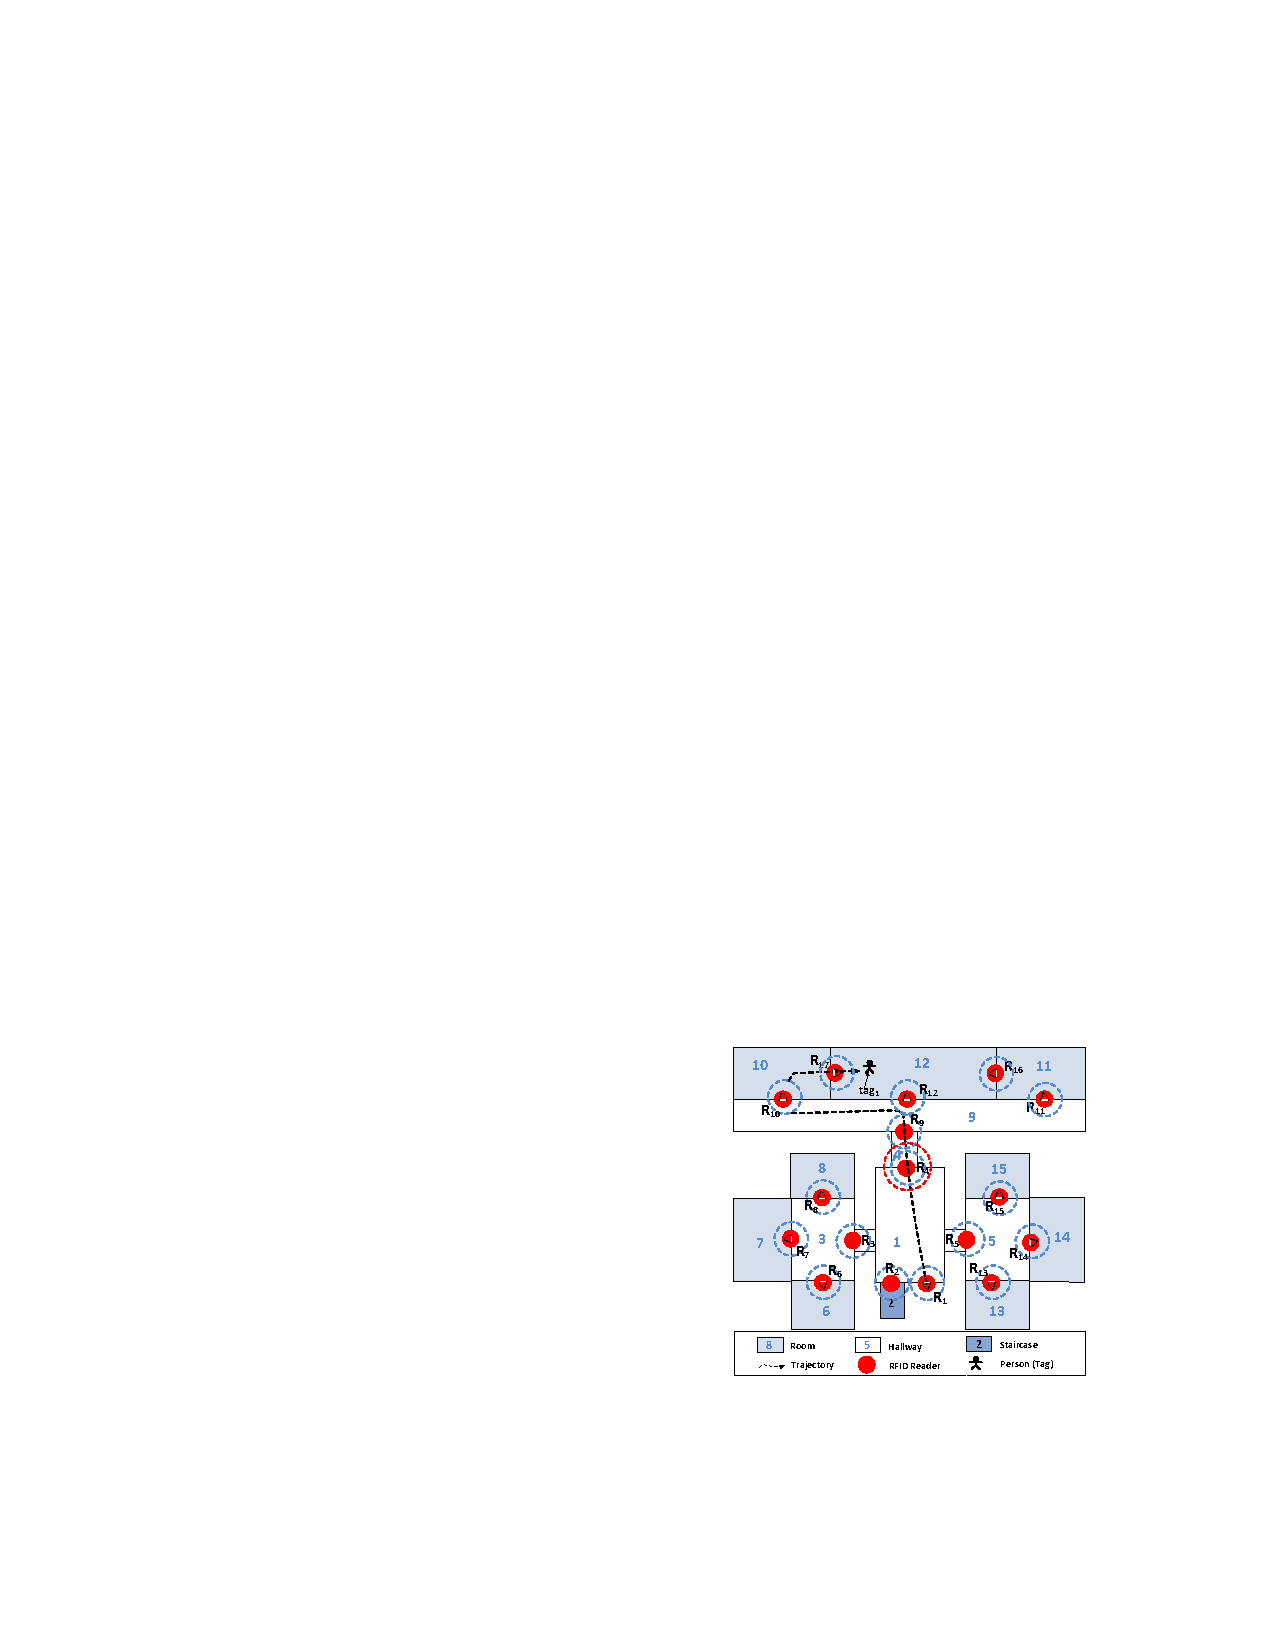
\includegraphics[width=0.75\columnwidth]{figures/3-5/3-5-1.pdf}
  \end{figure}
  \vspace{-20pt}
  \begin{figure}[tb]
    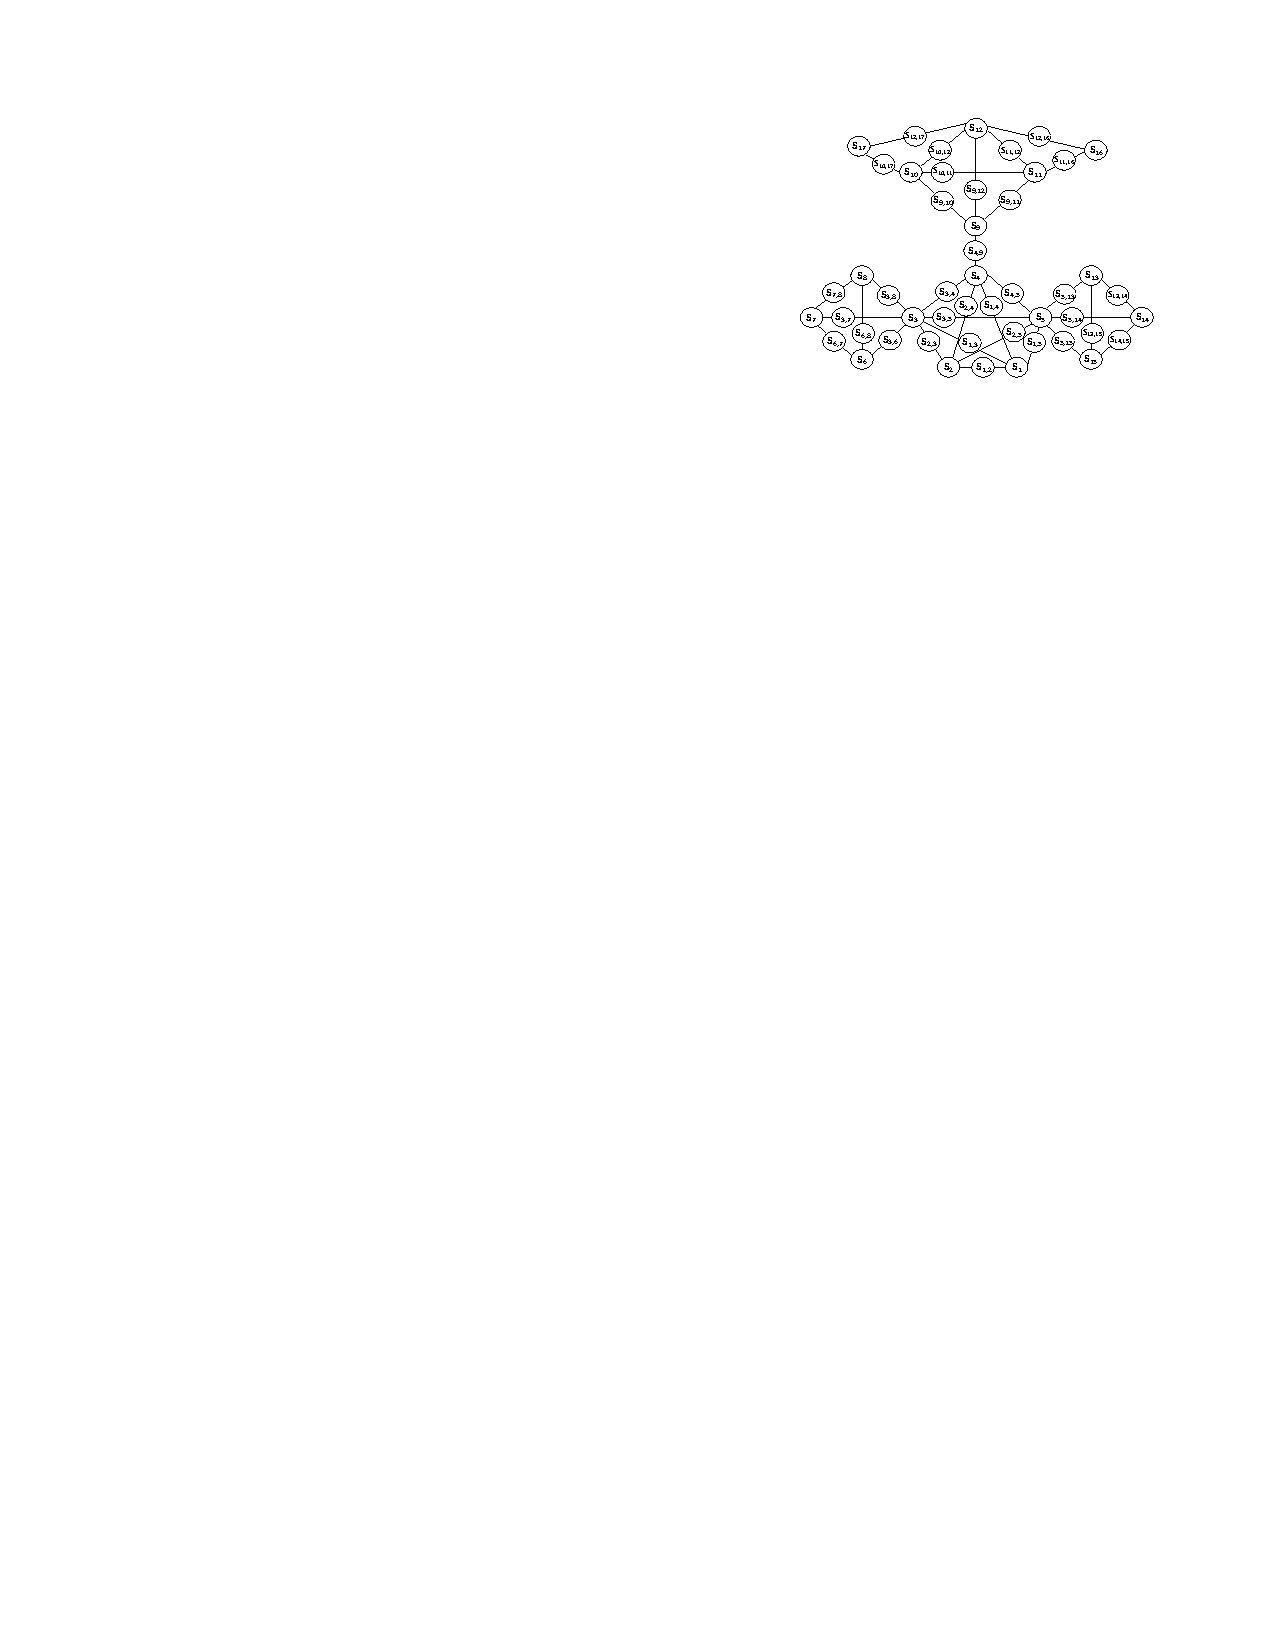
\includegraphics[width=0.75\columnwidth]{figures/3-5/3-5-8.pdf}
  \end{figure}

  \column{0.6\textwidth}
  \ssize{
  \textrm{This design contains a state $s_i$ for each deployed reader $R_i$, and a state $s_{ij}$ for each pair of adjacent readers $R_i$ and $R_j$. The intended meaning of $S_{ij}$ is that the object is transitioning between $R_i$ and $R_j$ (in either direction). The transition probabilities are non-zero only between states $s_i$ and $s_{kj}$, where $i \in \{ k,j \}$}\\~\\
  \begin{example}
    In this design, the state space size is $N = 50$ in the example.
  \end{example}
  }
\end{columns}

\end{frame}

%------------------------------------------------

\begin{frame}
\frametitle{Construction: Learning Parameters of IR-MHMM}

\fsize{

\emph{Standard EM Algorithm} (Baum-Welch algorithm in HMM context) which operates on the full transition matrix $A$ is used. \\~\\

Parameter constraints (form $a_{ij}$) are integrated into the learning procedure: one only needs to initialize these parameters with zero values. \\~\\

In order to avoid ``division by zero'' error in practice, to initalize the constrained parameter with small values ($ > 0$, like 0.01).\\~\\

For a fixed $i$, the initial values of the remaining transition probabilities $a_{ij}$ are set uniformly, $\sum_{j=1}^Na_{ij}=1$.\\~\\

In all the state space designs, we have for each reader $R_i$ a designated state $s_i$ correponding to locations within $R_i$'s range. That is $b_{ii} = 1$ and $b_{ik} = 0$ (a soft version is to set $b_{ik} = 0.01$ and $b_{ii} = 1 - 0.01$ due to the presence of cross readings).\\~\\

}

\end{frame}

%------------------------------------------------

\begin{frame}
\frametitle{Data Cleansing}

\begin{columns}

  \column{0.5\textwidth}
  \begin{figure}[tb]
    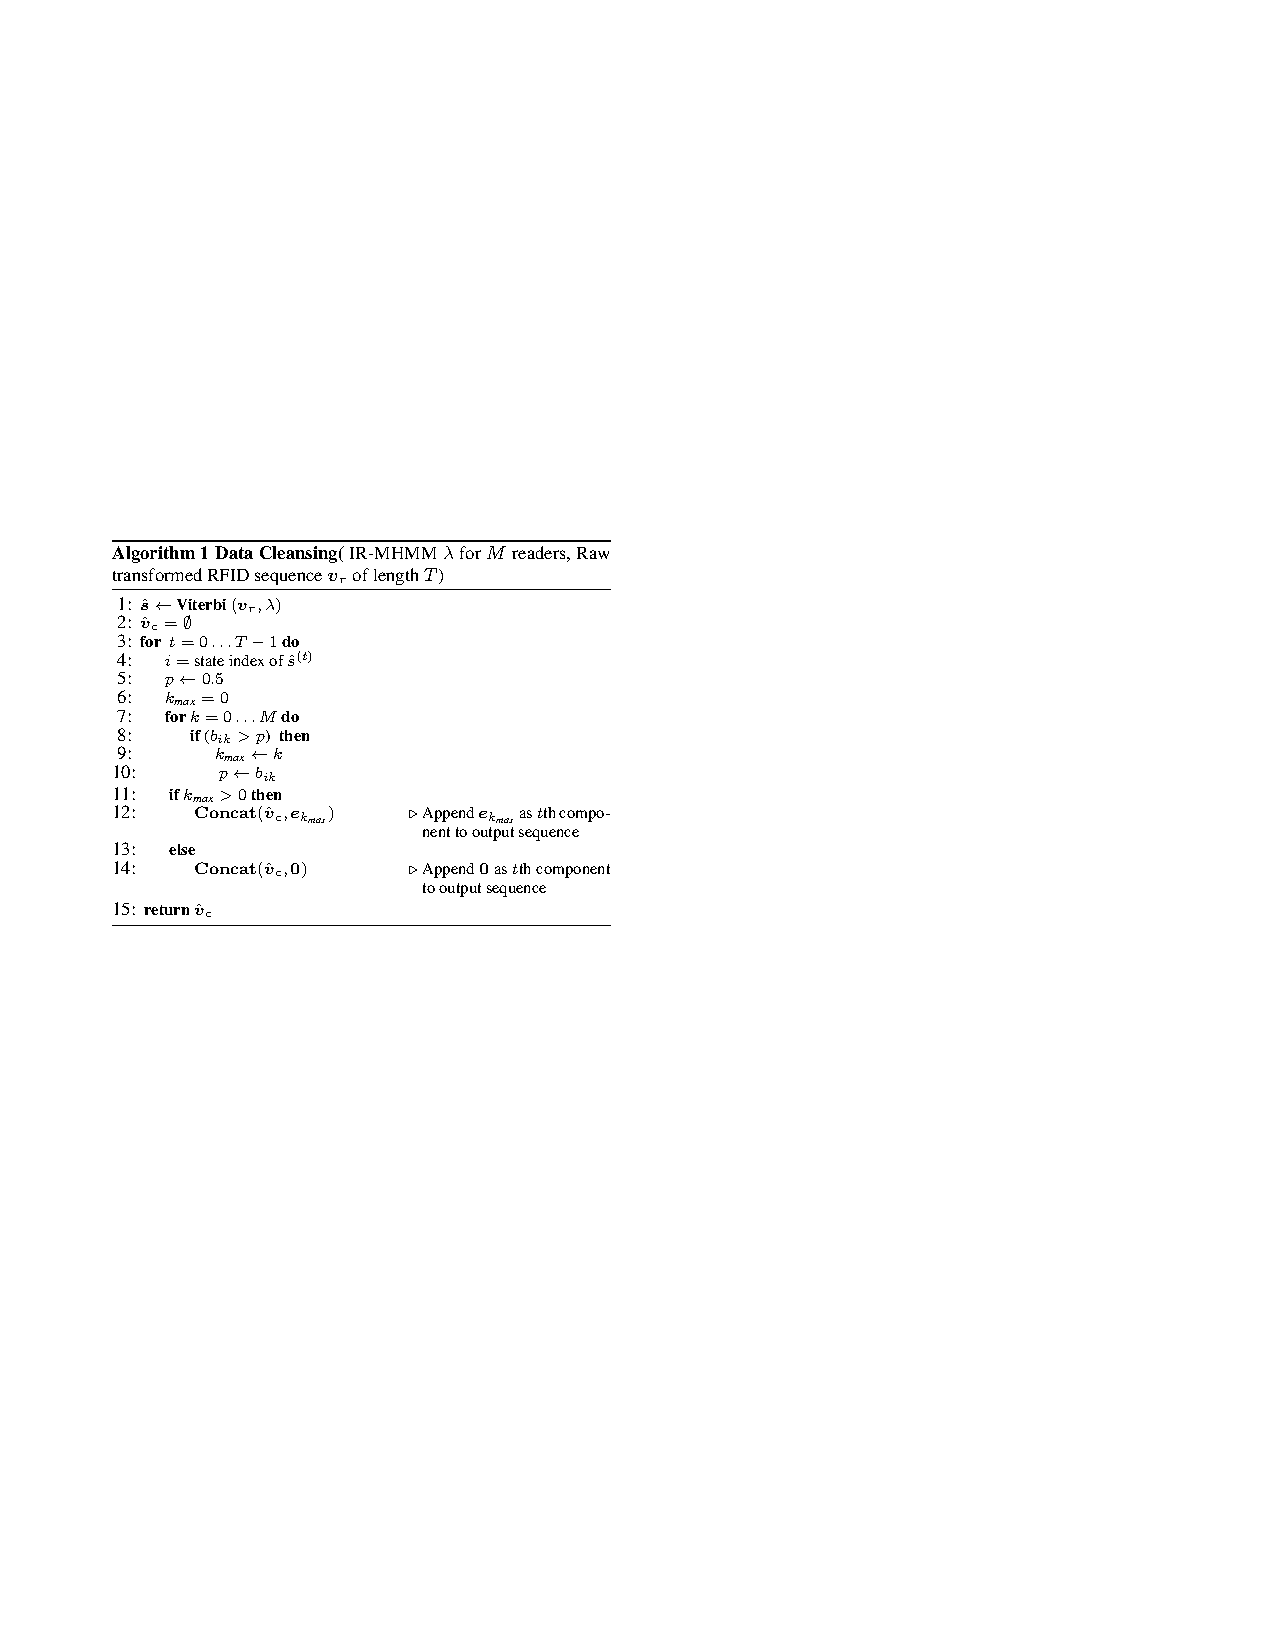
\includegraphics[width=\columnwidth]{figures/3-5/3-5-9.pdf}
  \end{figure}
  \ssize{\textit{input is raw RFID data transformed into a multi-variate binary observation sequence $\mathbf{v}_r = ( v_{r,1}^{(t)},...,v_{r,M}^{(t)} )_{t = 0,...,T-1}$, and an IR-MHMM $\lambda$.}}

  \column{0.6\textwidth}
  \begin{sitemize}
    \item first the standard Viterbi algorithm~\cite{viterbi1967error} is used to compute the most probable hidden state sequence $\mathbf{\hat{s}} = (\hat{s}^{(t)})_{t = 0,...,T-1}$.
    \item then compute the most probable observation sequence $\mathbf{\hat{v}_c} = (\hat{v}^{(t)}_{c,1},...,\hat{v}^{(t)}_{c,M})_{t = 0,...,T-1}$ given $\mathbf{\hat{s}}$, under the constraint that at each $t$, $(\hat{v}^{(t)}_{c,1},...,\hat{v}^{(t)}_{c,M})$ contains at most one non-zero entry.
    \item the most probable observation sequence given $\mathbf{\hat{s}}$ can be determined pointwise for each $t$ by maximizing $P(\mathbf{V}_r^({t}) = \mathbf{v}_r^{(t)} | S^{(t)} = \hat{s}^{(t)})$.
    \item if $\hat{s}^{(t)} = s_i$, then this probability is maximized by setting $\hat{v}^{(t)}_{r,k} = 1$ if $b_{ik} > 0.5$ otherwise $\hat{v}^{(t)}_{r,k} = 0$.
  \end{sitemize}

\end{columns}

\end{frame}

%------------------------------------------------

\begin{frame}
\frametitle{Edit Distance Based Evaluation}

To use a sequence of reader IDs to represent an object's trajectory. If there is no reading at a time point, symbol 0 is used; if there are more than one reading at a time point, a set of reader IDs are used. Raw and ground truth trajectory are shown in below figure.

\begin{figure}[tb]
  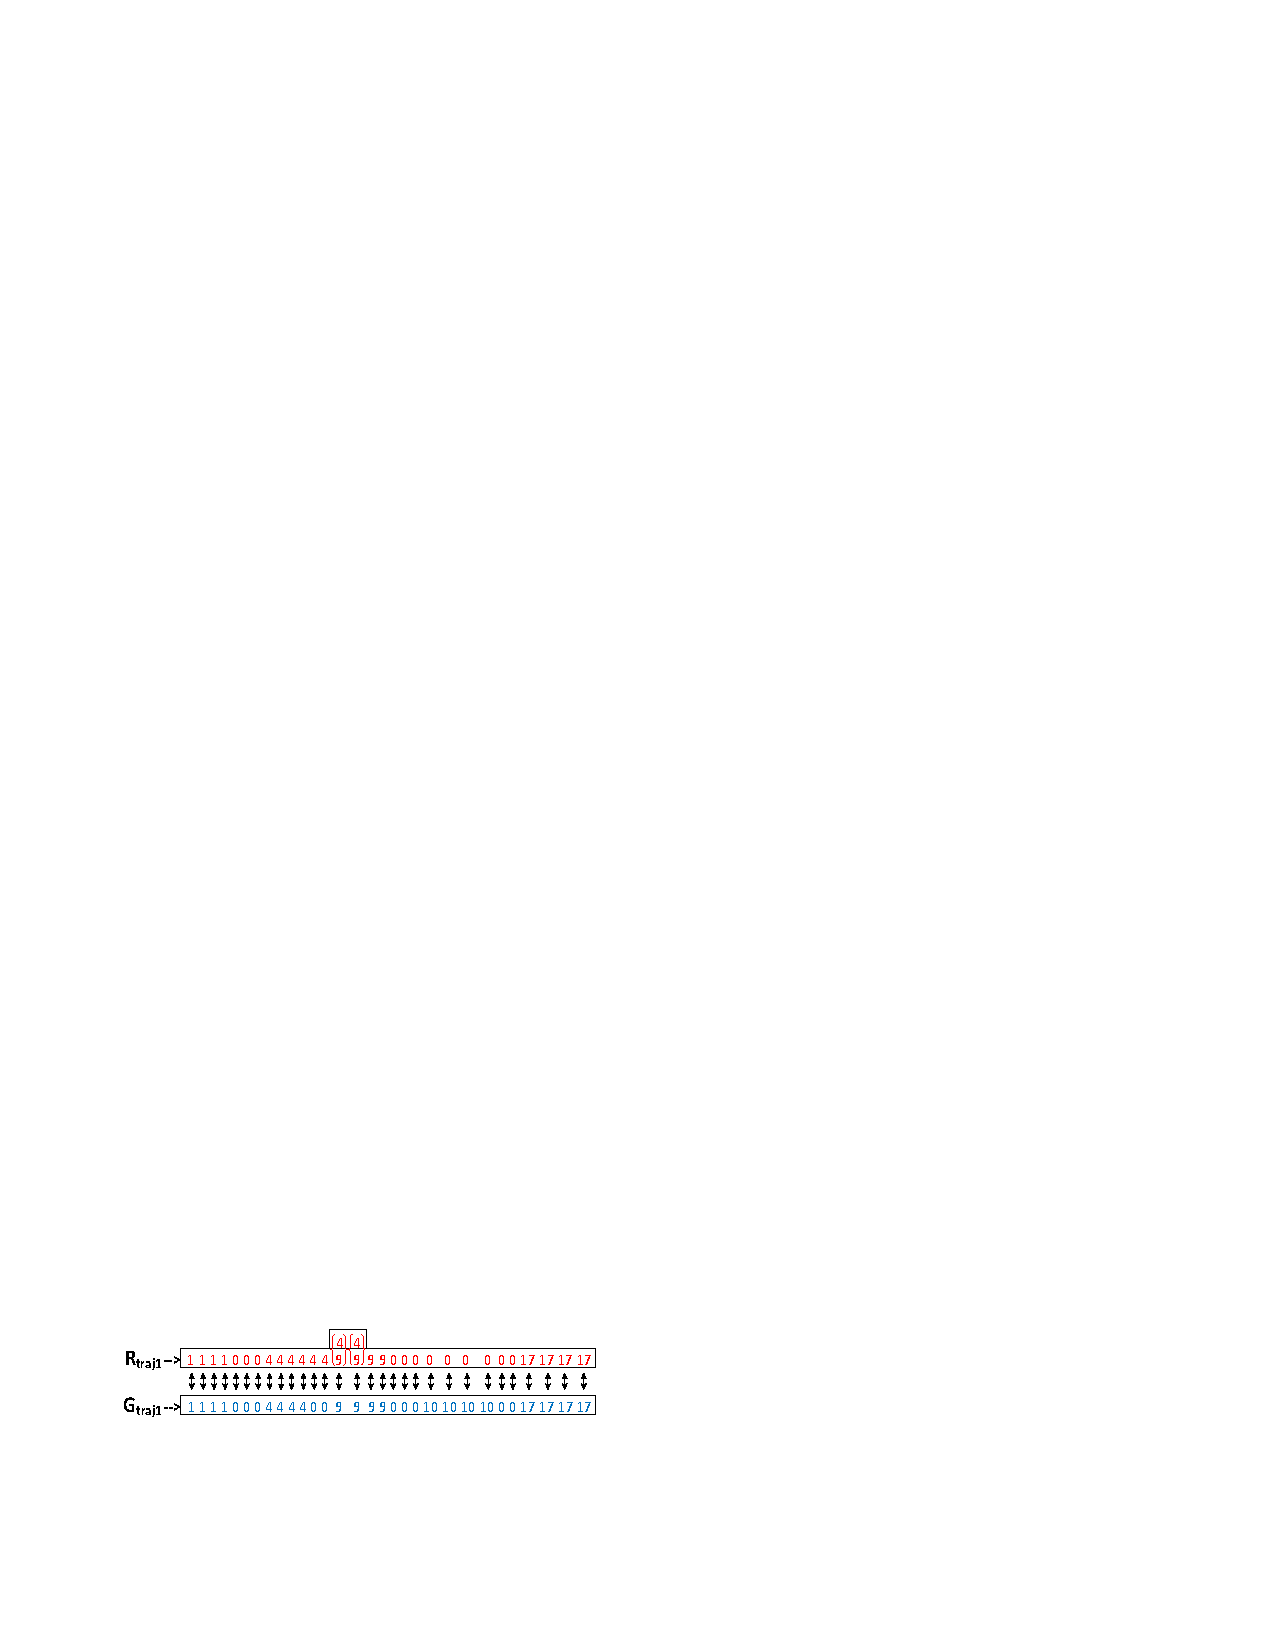
\includegraphics[width=\columnwidth]{figures/3-5/3-5-10.pdf}
\end{figure}

\end{frame}

%------------------------------------------------

\begin{frame}
\frametitle{Edit Distance Based Evaluation}

\ssize{

\conceptbf{Weighted Edit Distance Method} \quad allows the cost of a substitution to depend upon the symbols that are detected or inserted.\\~\\

For a substitution of a symbol set $\{ i,j \}$ with $i$ or $j$ we assign a cost of \conceptbf{1}, whereas a substitution with $k \neq i,j$ incurs a cost of \conceptbf{2}. Any insertion or deletion has a cost of \conceptbf{2}. \\~\\

\begin{figure}[tb]
  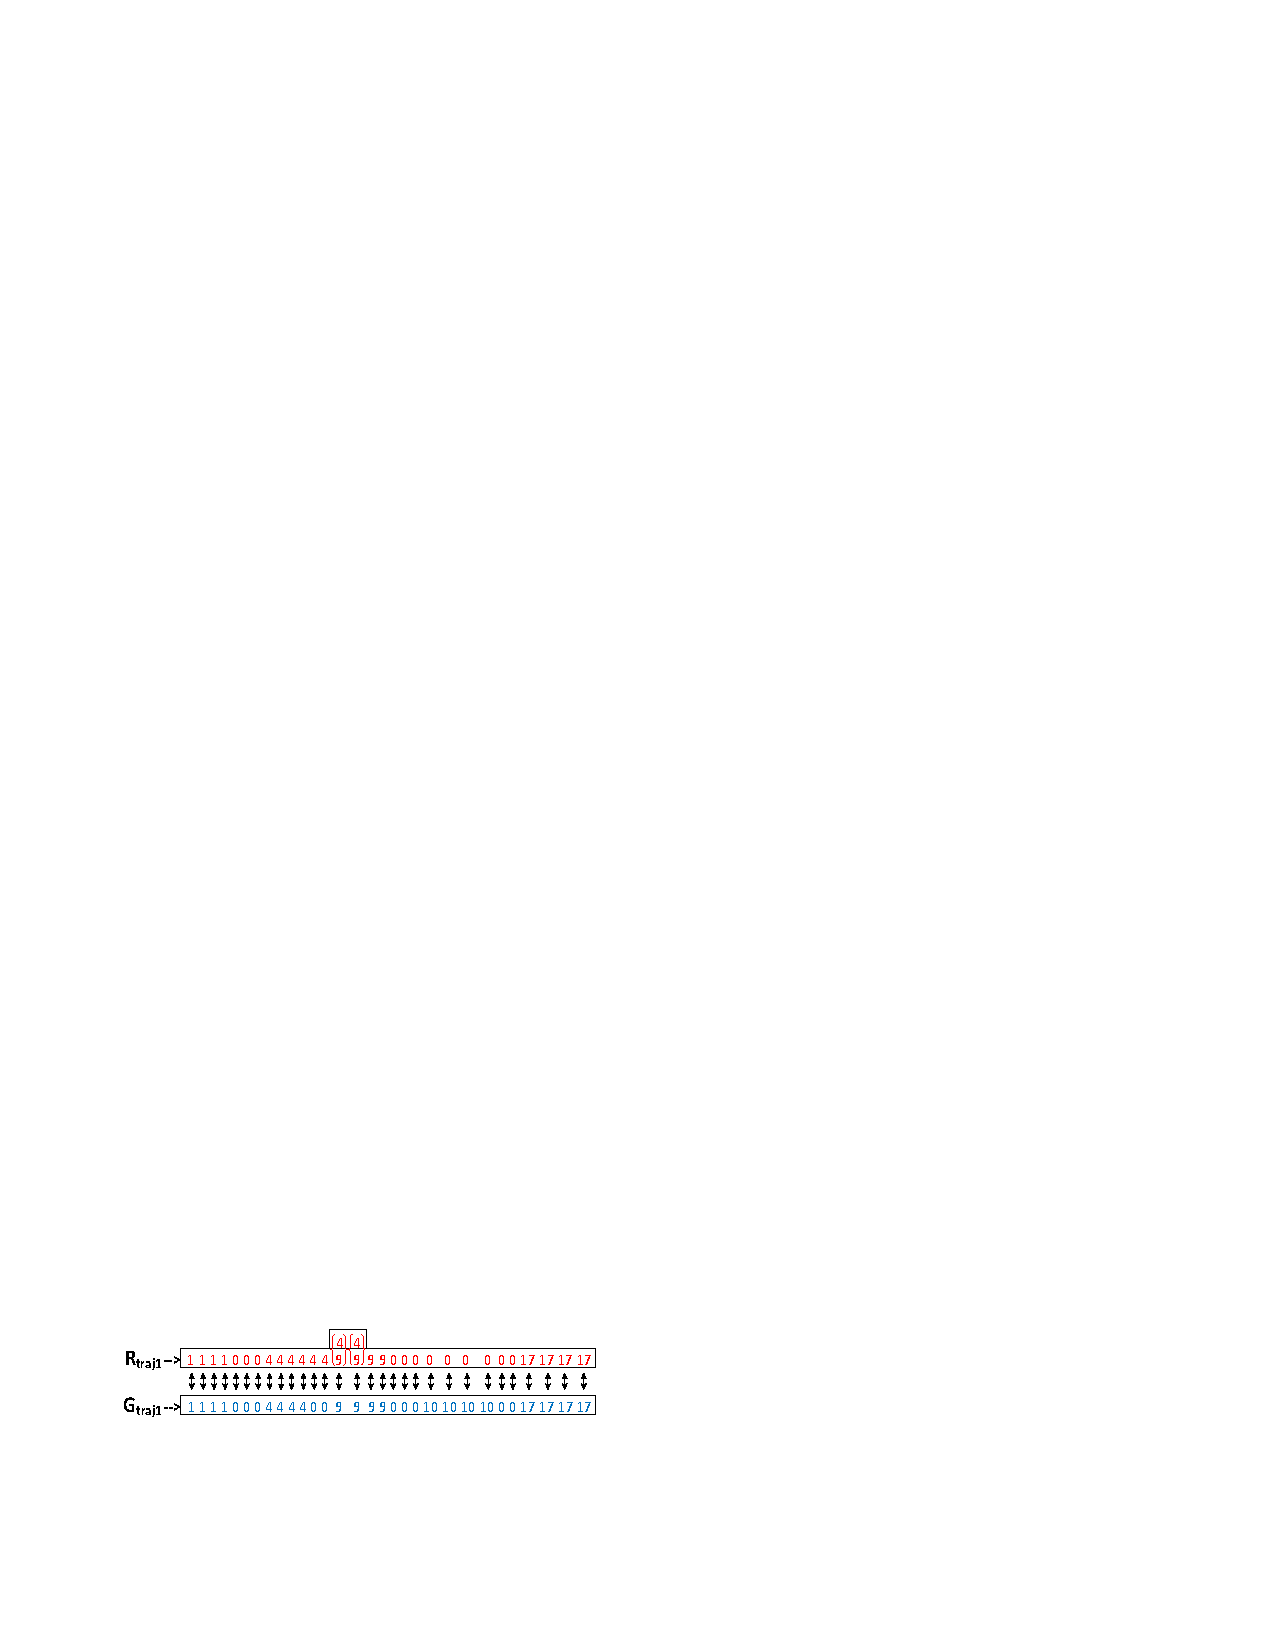
\includegraphics[width=\columnwidth]{figures/3-5/3-5-10.pdf}
\end{figure}

For the running example, compare ``$\{ 9,4 \}$'' with ``$9$'' and do the edit operation with an edit cost of 1. This leads to a much fairer evaluation, considering that one correct observation along with one wrong observation is still better than having two completely wrong observations.

}

\end{frame}

%------------------------------------------------

\begin{frame}
\frametitle{Edit Distance Computation Method 1}

To apply a weighted edit distance measurement to the original inferred observation sequence and the ground truth sequence.\\~\\

Not only check if the correct observation symbol is inferred but also check if it is correctly inferred at each time point.

\end{frame}
